%!TEX root = ../thesis.tex

\chapter{闪电氮氧化物的产率估算} \label{chapter:PE}

\section{清洁地区(北极)}

\subsection{闪电的分布} \label{subsect:lightning_distribution}

气候变暖正在引发全球闪电的变化\citep{Reeve.1999,Williams.2005a,Price.2009a}。
在过去的 30 年中,研究学者针对闪电预测提出了多种模拟方案\citep{Price.1992,Price.1997b,Allen.2002,Futyan.2007,Finney.2014,Romps.2014}。
气候模式结果显示,中纬度地区的闪电有所增加\citep{Michalon.1999,Romps.2014,Luhar.2021},
而在热带地区不同方案的预测结果目前仍存在分歧\citep{Finney.2018,Romps.2019}。
此外,虽然北极地区的变暖速度是全球平均水平的四倍\citep{Rantanen.2022},但针对北极闪电的研究还很少。
最近,\citet{Chen.2021a}针对北极地区开发了一个闪电参数化方案,结果表明,到本世纪末若全球平均气温上升3.7$^{\circ}$C,永冻区的闪电将增加74\%--150\%。
地基闪电观测结果显示,从 2010 年到 2020 年北极闪电占全球闪电的比例增加了三倍\citep{Holzworth.2021}。
此外,北极地区夏季更多的水汽辐合将加强对流系统,从而导致更多闪电\citep{Bintanja.2020}。

为了研究北极地区的闪电变化,我们将光学瞬态探测器(OTD, 1996--1999)\citep{Christian.2003} 的卫星闪电数据与维萨拉全球地基雷电数据集(GLD360,2019--2021)进行比较。
其中OTD仪器的观测范围为75$^{\circ}$ N以南,且其数据产品只包含闪电次数,一次闪电可包含一个或多个闪击。
虽然GLD360官方产品只包含闪击,但是我们的目的是研究闪电分布的变化,故未将闪击聚类成闪电。
GLD360数据覆盖了整个高纬度地区($>$60$^{\circ}$ N),而OTD仪器只观测到75$^{\circ}$ N以南的闪电。
在2019--2021年夏季(6月至8月), GLD360探测到75$^{\circ}$ N 以北发生的闪击所占比例为3\%(图\ref{fig:gld360_tseries})。

\begin{figure}[!htbp]
\centering
\includegraphics[width=12cm]{./figures/arctic_gld360_tseries.pdf}
\caption{
GLD360探测的每10分钟闪击时间序列。\\
Figure \ref{fig:gld360_tseries}. Time series of GLD360 lightning strokes per 10 minutes.
}
\label{fig:gld360_tseries}
\end{figure}


在图\ref{fig:arctic_lightning_distribution} 中,我们使用卫星和地面闪电观测比较了高纬度地区夏季(6--8 月)闪电的空间分布。
两个数据集都显示西伯利亚和阿拉斯加永冻区具有较高的闪电频率(60$^{\circ}$--65$^{\circ}$ N,图\ref{fig:arctic_lightning_distribution}(a) 和 \ref{fig:arctic_lightning_distribution} (b)),这是北极火灾的主要来源\citep{McCarty.2021}。
OTD 平均闪电频率和 GLD360 平均闪击频率分别为 0.22 km$^{-2}$ 每月 和 0.61 km$^{-2}$ 每月。
然而,OTD 在楚科奇海(Chukchi Sea)附近记录的闪电较少,但在伊明格海(Irminger Sea)上空较多。
这种现象归因于北极降水的年际变化,与向极地输送的水汽有关\citep{Bintanja.2020}。

为了判断 TROPOMI 是否可以探测到 LNO$_2$,我们首先计算了每次TROPOMI过境前3 h内发生在条带里的GLD360闪电数。
虽然TROPOMI不会连续对北极进行探测,但在夏季该地区每天有14个重叠轨道,从而覆盖了北极的大部分地区。
TROPOMI条带内的闪击数约占总计数的 9\%(图\ref{fig:arctic_lightning_distribution}c),并且它们具有相同的地理分布(图\ref{fig:arctic_lightning_distribution}b)。
由于在高纬度地区有更多的重叠条带,条带内闪击的比例随着纬度增大而增大(图\ref{fig:arctic_lightning_distribution}d),从$<$ 10\% (60$^{\circ}$--70$^{\circ}$ N) 增加到 10\%--25\% (70 $^{\circ}$--80$^{\circ}$ N) 和 40\%--100\%(80$^{\circ}$--90$^{\circ}$ N)。
而地基观测\citep{Schmale.2018} 和飞机观测\citep{Jacob.2010}的NO$_2$数据有限,因此TROPOMI的NO$_2$卫星观测数据在分析北极的 LNO$_2$ 方面非常有利。
鉴于 70$^{\circ}$ N 以北具有更高的 TROPOMI 覆盖率和更少的其他NO$_2$排放源(例如野火或天然气),我们选择该区域来计算LNO$_2$ 产率(PE)。
GLD360在70$^{\circ}$ N 以北探测到的夏季(6--8 月)闪击数分别为 1.2$\cdot$10$^6$ (2019)、1.6$\cdot$10$^6$ (2020) 和 9.8$\cdot$10$^5$ ( 2021)(表\ref{table:arctic_emission})。
其中在TROPOMI 覆盖率最高的地区(80$^{\circ}$--90$^{\circ}$ N),2021 年的闪击数约为 2.9$\cdot$10$^4$,是前九年总数的近两倍\citep{networktotal.2021}。
最北端可达89.5$^{\circ}$ N,世界闪电定位网络 (WWLLN)也探测到了该闪击(89.6 $^{\circ}$ N)\citep{Holzworth.2021}。


\begin{figure}[htbp]
\centering
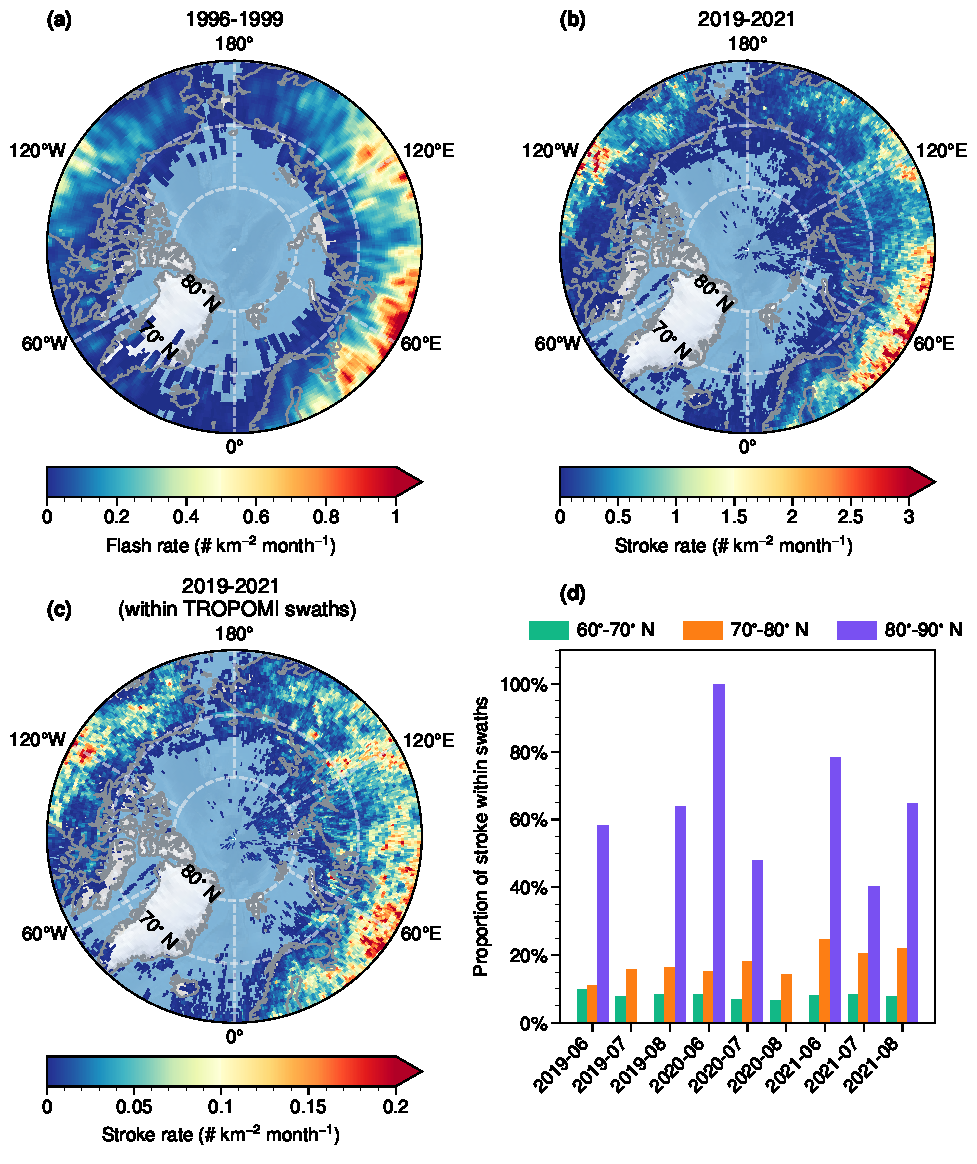
\includegraphics[width=10.5cm]{./figures/arctic_lightning_distribution.pdf}
\caption{
(a) 1996--1999年6--8月OTD平均闪电频率;
(b) 2019--2021年6--8月GLD360平均闪击率;
(c) 与 (b) 相同,但只计算 TROPOMI 过境前 6 h内 TROPOMI 条带内的闪电。
没有闪电的网格在 (a)--(c) 子图中设置为淡蓝色。
(d) (c) 与 (b) 的月比例。\\
Figure \ref{fig:arctic_lightning_distribution}.
(a) Mean OTD lightning flash rate over June--August of 1996--1999;
(b) Mean GLD360 lightning stroke rate over June--August of 2019--2021;
(c) Same as (b) but only counting the lightning inside the TROPOMI swaths during the 3-hour period before the TROPOMI overpass time.
Grids with no lightning appear as the light-blue backgrounds in (a)--(c) panels.
(d) The monthly ratio of (c) to (b).
}
\label{fig:arctic_lightning_distribution}
\end{figure}


\begin{table*}
\centering
\caption{2019--2021期间高纬度地区GLD360探测到的闪击数、闪电NO$_2$排放(Mg[N])和平均对流有效位能(CAPE, J kg$^{-1}$)\\
Table \ref{table:arctic_emission}. GLD360 stroke counts, lightning NO$_2$ (LNO$_2$) emissions (Mg[N]), and mean Convective available potential energy (CAPE, J kg$^{-1}$) in the Arctic region for the June--August periods of 2019--2021.
}
\label{table:arctic_emission}
\begin{tabular}{rrrrrr}
\hline
{} & 70$^{\circ}$--75$^{\circ}$ N & 75$^{\circ}$--80$^{\circ}$ N &
80$^{\circ}$--85$^{\circ}$ N &  85$^{\circ}$--90$^{\circ}$ N &  \\
\hline
Strokes & & & & & Total \\
\hline
2019 &   1,142,292 &     40,660 &      5,756 &       636  & 1,189,344 \\
2020 &   1,402,304 &    233,780 &      4,784 &       768  &  1,641,636 \\
2021 &     889,248 &     62,296 &     26,576 &      2,536  &  980,656 \\
\hline
LNO$_2$ & & & & & Total \\
\hline
2019 &      87.3 &       5.6 &       0.9 &       0.1 &   93.9 \\
2020 &      85.5 &      22.1 &       0.8 &       0.1 &  108.5 \\
2021 &      58.6 &       8.6 &       3.9 &       0.4 &   71.5 \\
\hline
CAPE & & & & & Mean \\
\hline
2019 & 5.5  & 4.0  & 5.0  & 6.5 & 5.3 \\
2020 & 9.2  & 5.1  & 5.0  & 5.2 & 6.1 \\
2021 & 7.3  & 4.8  & 5.5  & 7.2 & 6.2 \\
\hline
\end{tabular}
\end{table*}


\subsection{闪电氮氧化物的反演}

LNO$_2$的估算包括以下三个主要步骤:

1. 使用风场数据将NO$_2$柱密度高值区与闪电数据匹配。

2. 基于新算法来计算LNO$_2$柱密度。

3. 使用连续的TROPOMI观测数据来计算LNO$_2$的产率。

\subsection*{闪电的聚类}

我们使用具有噪声的基于密度的聚类方法(DBSCAN)将TROPOMI过境前12 h内\citep{Allen.2021a}的闪击以40km进行聚类\citep{backlund2011density,Schubert.2017}。
由于野火也会产生 NO$_2$,因此使用可见光/红外成像仪/辐射计套件(VIIRS)375 m 主动火点产品,来识别和过滤受野火排放影响的闪电聚类。
VIIRS 搭载在 Suomi 国家极地轨道合作伙伴 (Suomi-NPP) 上,它与搭载TROPOMI的S5P在同一轨道上,但比 S5P 提前 3.5 分钟。
我们将内部没有火点的闪电集群视为一个清洁的聚类。

对于每个清洁的闪电聚类,我们根据观测到的闪击所在位置及时间来在三个气压层(300 hPa、500 hPa 和 700 hPa)上定义受 LNO$_2$ 影响的空气块(图 \ref{fig:workflow}a)。
如图 \ref{fig:workflow}b 所示,含 LNO$_2$ 的空气块通过水平平流传输。
为了确定 TROPOMI 过境时空气块的位置,我们使用 ECMWF 小时大气再分析资料(ERA5) 的风场数据\citep{Hersbach.2020}。
最终的空气块组合成一个闪电掩膜(图 \ref{fig:workflow}c中的橙色圆圈),即三个等压面的前向轨迹构成了一个近似的 LNO$_2$ 区域。

我们首先使用分水岭方法得到NO$_2$垂直柱密度($V_{\ch{NO2}}$)的高值区(图 \ref{fig:workflow}(c)中的像素)。
具体而言,分水岭方法将输入数据视为地形表面,并将它们分成单独的区域,称为集水盆地\citep{Soille.1990,Heikenfeld.2019a}。
在本研究中,我们应用从 4$\cdot$10$^{14}$ 到 1$\cdot$10$^{15}$ molec. cm$^{-2}$ 的阈值,步长为 2$\cdot$10$^{14}$ molec. cm$^{-2}$来检测多个局部高 NO$_2$ 特征。
这些特征用于识别具有高 $V_{\ch{NO2}}$ 的附近区域(图 \ref{fig:workflow}c 中不同颜色的像素)。
我们选择包含一个或多个高 $V_{\ch{NO2}}$ 区域的聚类用于 LNO$_2$ 的进一步分析。
最终对闪电掩膜内的数据用分水岭方法进行重新识别,得到具有高 $V_{\ch{NO2}}$ 的LNO$_2$ 区域(图 \ref{fig:workflow}d 中的亮色像素)。

在重新使用分水岭方法之前,我们使用最小-最大归一化将掩膜内的 $V_{\ch{NO2}}$ 值归一化为 0 到 1 的范围,即从每个数据中减去最小值并除以最大值和最小值之间的差值。
我们将对数正态分布模型拟合到置信度为 80\% 的归一化值,并将结果用作分水岭过程的最小阈值。
由于 LNO$_2$ 区域通常小于闪电掩模(图 \ref{fig:workflow}d),
80\% 的置信水平应该足以识别 LNO$_2$ 像素。
与置信度相关的不确定性结果记录在表 \ref{table:arctic_uncertainty} 中。
最后,我们将分水岭算法应用于标准化的 $V_{\ch{NO2}}$ 值,使用的阈值范围从最小值到 1,步长为 10,
这使我们能够识别和分析最终的LNO$_2$数据。


\begin{figure}[htbp]
\centering
\includegraphics[width=14cm]{./figures/arctic_workflow.pdf}
\caption{
从 TROPOMI 轨道 09458(2019 年 8 月 1 日)数据选择闪电 NO$_2$ 像素的示意图。
背景填色为TROPOMI 检测到的 NO$_2$ 对流层柱, (a) 观测到的闪击,
(b) 在三个气压层(300 hPa、500 hPa 和 700 hPa)上水平传输的闪电 NO$_2$ 空气块,
(c) 将空气块组合成一个闪电掩膜(橙色圆圈),高 NO$_2$高值区(填充像素)重叠。
不同的像素颜色代表基于多个 NO$_2$ 阈值的不同 NO$_2$ 选区。
(d) 掩膜内受闪电 NO$_2$ 影响的 NO$_2$ 对流层柱密度的最终选区(亮色像素)。\\
Figure \ref{fig:workflow}. Overview of the process for identifying lightning NO$_2$ pixels from TROPOMI orbit 09458 on August 1, 2019.
The TROPOMI-detected NO$_2$ tropospheric columns are overlaid with (a) observed lightning strokes and
(b) transported air parcels of lightning NO$_2$ at three pressure levels (300 hPa [blue], 500 hPa [orange], and 700 hPa [green]).
(c) Parcels are combined into one lightning mask (orange circle), which overlaps with high NO$_2$ selections (filled pixels). The different pixel colors represent different NO$_2$ selections based on multiple NO$_2$ thresholds.
(d) The final selection (bright colored pixels) of NO$_2$ tropospheric columns affected by lightning NO$_2$ within the mask.
}
\label{fig:workflow}
\end{figure}

\subsection*{计算闪电氮氧化物柱密度}

正如\citet{Zhang.2022a}中所讨论的,官方 TROPOMI 算法在 NO$_2$反演中不包括 LNO$_2$。
因此,我们从官方 S$_{\textrm{NO$_2$}}$产品中减去背景 NO$_2$,并将差值通过空气质量因子 (AMF) 转换为对流层LNO$_2$垂直柱密度。
该算法具体为下式


\begin{equation} \label{eq:arctic_LNO2}
V_{\ch{LNO_2}} = \frac{S_{\ch{NO_2}} - S_{\ch{BG}}}{AMF_{\ch{LNO_2}}}
\end{equation}


其中 $V_{\ch{LNO2}}$ 是对流层 LNO$_2$ 垂直柱密度,
$S_{\ch{NO2}}$ 是 TROPOMI 测得的对流层 NO$_2$ 斜柱密度,
$AMF_{\ch{LNO2}}$ 是新定义的闪电空气质量因子。
根据\citet{Allen.2021a}的研究,我们将背景 $S_{\ch{NO2}}$($S_{\ch{BG}}$)定义为对流层 AMF 和在闪电掩膜内NO$_2$低值区的第 30 个百分位数$V_{\ch{NO2}}$的乘积。
NO$_2$低值区(图 \ref{fig:workflow}(d)中的灰色像素)是由分水岭技术得到的$V_{\ch{NO2}}$高值区之外的所有掩膜像素。
$AMF_{\ch{LNO2}}$ 是“可见”LNO$_2$ 斜柱密度与对流层 LNO$_2$ 垂直柱密度之比:

\begin{equation} \label{eq:arctic_AMFLNO2}
AMF_{\ch{LNO_2}} = \frac{(1-f_r) \int_{p_{surf}}^{p_{tp}} w_{clear}(p) LNO_2(p) \: dp + f_r \int_{p_{cloud}}^{p_{tp}} w_{cloudy}(p) LNO_2(p) \: dp}{\int_{p_{surf}}^{p_{tp}} LNO_2(p) \: dp}
\end{equation}

其中 $f_{r}$ 是 NO$_2$ 窗口中的云辐射率分数,
$p_{surf}$ 是表面压力,
$p_{cloud}$ 是云压力,
$p_{tp}$ 是对流层顶压力,
$w_{clear}$ 和 $w_{cloudy}$ 分别是来自查找表 \cite{Lorente.2017} 的晴天和多云部分的压力相关散射权重,
$LNO_2(p)$ 是由修正的高斯分布呈现的与压力相关的对流层 NO$_2$ 剖面。
\citeauthor{Ott.2010} \cite{Ott.2010} 和 \citeauthor{Luo.2017} \cite{Luo.2017} 高斯分布的峰宽设置为180 hPa(详见补充),以及 峰值水平是闪电面罩中最高的 TROPOMI 云压。

其中 $f_{r}$ 是NO$_2$窗区的云辐射率分数,
$p_{surf}$ 是地表气压,
$p_{cloud}$ 是云压,
$p_{tp}$ 是对流层顶气压,
$w_{clear}$ 和 $w_{cloudy}$ 分别是来自查找表 \citep{Lorente.2017}的晴天和多云部分的与气压有关的散射权重,
$LNO_2(p)$ 是与气压有关的高斯分布先验 LNO$_2$廓线。
我们将高斯分布的峰值高度设置为闪电掩模中最高的TROPOMI云压,峰值宽度设置为180 hPa。
该峰值宽度是通过利用高斯分布拟合前人的LNO$_x$廓线得到的,具体如下。
高斯分布由方程 $k*e^\frac{{-{(p - peak\_pressure)}^2}}{2*peak\_width^{2}}$ 给出。
在这个等式中,系数 $k$ 在 AMF 计算中同为分子和分母所以被抵消,$p$ 是TM5-MP的气压层。
利用该公式拟合 \citet{Ott.2010} 的海洋LNO$_x$廓线和\citet{Luo.2017}的中纬度大陆LNO$_x$廓线,得到$peak\_width$ 的平均值为180 hPa(图\ref{fig:arctic_lnox_profile})。
没有使用\citet{Ott.2010}中的中纬度大陆 LNO$_x$ 廓线,是由于\citet{Luo.2017}指出该廓线与对流前的廓线相似,而我们需要对流时的廓线。
表 \ref{table:arctic_uncertainty} 总结了与 $peak\_width$ 和云压相关的 LNO$_2$ 生产效率的不确定性。

\begin{figure}[ht]
\centering
\includegraphics[width=16cm]{./figures/arctic_lnox_profile.pdf}
\caption{
每公里LNO$_x$质量百分比的平均垂直分布。
数据来源:(a) \citet{Pickering.1998} 和 (b) \citet{Ott.2010}。
来自 \citet{Luo.2017} 的 LNO$_x$ 配置文件以黑色显示。
(c) 高斯拟合曲线(虚线)和原始数据(散点)。\\
Figure \ref{fig:arctic_lnox_profile}.
Average vertical distributions of percentage of typical LNO$_x$ mass per kilometer.
The LNO$_x$ profiles shown are from (a) \citet{Pickering.1998} and (b) \citet{Ott.2010}.
The LNO$_x$ profile from \citet{Luo.2017} is shown in black.
(c) The Gaussian fitting profiles (dashed lines) and the original data (scatter points).
}
\label{fig:arctic_lnox_profile}
\end{figure}

$AMF_{\ch{LNO2}}$计算中使用的散射权重由五个参数决定:地表气压、太阳天顶角、观察天顶角、相对方位角和反照率。
对于多云部分,查找表中使用的地表气压和反照率值则针对云而设定,即地表气压等于云压力,反照率等于云反照率。
TROPOMI 检测到的云压代表云内部的气压水平,而不是几何云顶\citep{Vasilkov.2008,Joiner.2012}。
它的范围从 130 hPa 到 987 hPa,最常见的值在 250--300 hPa 区间(图\ref{fig:pcld_ptropo})。
由于因为 NO$_2$ 高值在云内部,而云上方的 NO$_2$ 由于光解作用浓度较低 \citep{Beirle.2009},
所以高斯分布的 LNO$_2$ 扩线应比默认的先验 NO$_2$ 廓线更准确,
对于又高又厚的云层,云层上方的散射权重相当均匀,并且LNO$_2$的灵敏度在云中部附近最高,与 TROPOMI测到得的云压接近\citep{Beirle.2009}。
这最大限度地减少了可能错误假设的 NO$_2$ 峰值气压对反演的影响\citep{Laughner.2017}。
此外,我们剔除了云层高于对流层顶的个例,因为 NO$_2$ 浓度可能会受到平流层 O$_3$ 的影响\citep{Frey.2015a,Zhang.2022a}


\subsection*{计算闪电氮氧化物产率} \label{sec:calc_lnox_pe}

如\ref{subsect:lightning_distribution}节所述,TROPOMI 可多次扫过 70$^{\circ}$ N 以北的同一点。
因此,两个连续的轨道可以观测到相同的雷暴。
为了更轻松地分析北极 LNO$_2$ 案例的模式和变化,我们创建了一个交互式网站 (\url{https://arctic-lightning-no2.streamlit.app/}),允许用户筛选个例和以交互的方式研究LNO$_2$、云压和闪电之间的关系。

$V_{\textrm{LNO$_2$}}$ (mol m$^{-2}$) 在相邻过境时间之间的关系可以定义为

\begin{equation} \label{eq:relationship}
\sum_{p_{(T2)}} V_{\ch{LNO_2_i}} A_{i} = e^\frac{{-(T_2-T_1)}}{\tau} \sum_{p_{(T1)}} V_{\ch{LNO_2_j}} A_{j} + PE \sum_{N} e^\frac{{-(T_2-t_k)}}{\tau}
\end{equation}


其中 $p$ 是 LNO$_2$ 区域中的像素数,
$A$ 是每个像素的面积(m$^2$),
$T$ 是 TROPOMI 过境时间,
$t$ 是闪电发生的时间,
$\tau$ 是对流附近 LNO$_2$ 的寿命,
$PE$ 是 LNO$_2$ 的产率 (mol stroke$^{-1}$),
$N$ 是发生在相邻过境时间内的总闪击数,
而指数成分考虑了 NO$_2$ 的化学损失。
除此之外,$i$ 和 $j$ 是 TROPOMI 的像素索引,
$A_{i}$ 和 $A_{j}$ 是不同的 LNO$_2$ 区域,并考虑了平流的影响(图\ref{fig:consecutive_orbits}),
$T_1$ 和 $T_2$ 表示 TROPOMI 在 LNO$_2$ 区域的两次平均过境时间,
$t_k$ 表示两个轨道之间发生的第 k 次雷击(k 取值范围为 1 到 N)的时间。


如果相邻过境时间内没有闪电发生,式(\ref{eq:relationship})可以简化为:

\begin{equation} \label{eq:LNO2_nolightning}
\sum_{p_{(T2)}} V_{\ch{LNO_2}_i} A_{i} = e^\frac{{-(T_2-T_1)}}{\tau} \sum_{p_{(T1)}} V_{\ch{LNO_2}_j} A_{j}
\end{equation}

我们通过分析具有高 LNO$_2$ 但两次过境时间之间没有闪电的特殊个例,得到 $\tau$ 的值为 3 $\pm$ 1 h(表\ref{table:lifetime} 和图 \ref{fig:consecutive_orbits}).
并将其代入方程 (\ref{eq:relationship}) 来计算剩余个例的 LNO$_2$ PE。


\begin{figure}[!htbp]
\centering
\includegraphics[width=13cm]{./figures/arctic_consecutive_orbits.pdf}
\caption{
受闪电 NO$_2$ 影响的 NO$_2$ 对流层柱密度的选区(亮色像素)。
(a--b) 两次连续的过境数据,且它们之间有活跃的闪电。
(c--d) 两次连续的过境数据,但它们之间没有闪电。\\
Figure \ref{fig:consecutive_orbits}. Selections (bright colored pixels) of NO$_2$ tropospheric columns affected by lightning NO$_2$.
(a--b) Two consecutive orbits with active lightning between them.
(c--d) Two consecutive orbits with no lightning between them.
}
\label{fig:consecutive_orbits}
\end{figure}


\begin{table}[!htbp]
\centering
\caption{2019--2021期间得到的闪电 NO$_2$ (LNO$_2$) 的寿命\\
Table \ref{table:lifetime}. Lightning NO$_2$ (LNO$_2$) lifetimes derived from cases (2019--2021).}
\label{table:lifetime}
\begin{tabular}{llllll}
\hline
时间             &         轨道 &    经度 &   纬度 &  $\Delta$面积 (\%) &  寿命 (h) \\
\hline
2019-06-28 00:38 &       08833 &  127.4 &  81.0 &     -14.5 &       3.0 \\
2019-08-14 22:58 &       09513 &  126.0 &  70.4 &       2.0 &       1.7 \\
2020-06-09 19:11 &       13767 &  162.8 &  73.0 &     -43.8 &       3.6 \\
2020-06-15 22:18 &       13854 &  155.6 &  78.7 &      -4.4 &       3.4 \\
2020-07-15 21:19 &       14279 &  109.3 &  75.4 &       4.5 &       2.7 \\
2021-07-11 11:40 &       19395 &  -84.5 &  70.9 &      28.0 &       5.2 \\
\hline
\end{tabular}
\footnotesize
\shortstack[l]{
$\Delta$面积 是 LNO$_2$ 面积在 $T_2$ 相对于 $T_1$ 的百分比变化 \\
($T_1$ 和 $T_2$ 是连续条带的平均过境时间,$T_2$ > $T_1$)。\\
$\Delta$Area is the percentage change of the LNO$_2$ area at $T_2$ relative to $T_1$ \\
($T_1$ and $T_2$ are the mean overpass time of consecutive swaths, $T_2$ > $T_1$).
}
\end{table}


在前人的研究中共有三种方法来估算热带和中纬度地区的 LNO$_2$ 产量:

(1)背景NO$_2$加上LNO$_2$(LNO$_2$$^*$)与闪电之间的线性回归 \citep{Pickering.2016,Allen.2019,Lapierre.2020};

(2)使用定义的空气质量因子直接得到NO$_2$ \citep{Beirle.2009,Zhang.2020b,Zhang.2022a};

(3)算出LNO$_2$$^*$并减去背景 NO$_2$,其中背景 NO$_2$取自飞机观测 \cite{Pickering.2016,Perez-Invernon.2022} 或未发生闪电的对流像素处的平均NO$_2$ \citep{Bucsela.2019,Bucsela.2010,Allen.2021a}。

由于背景 NO$_2$ 随太阳天顶角而变化,线性回归不适用于我们的情况。

第二种方法需要使用闪电参数化进行详细的 LNO$_2$ 模拟,而目前闪电参数化的不确定性仍非常大 \cite{Finney.2018,Romps.2019,Chen.2021a},尤其是在闪电数据集很少的北极地区 \citep{Holzworth.2021}。
最后一种方法需要的平均背景 NO$_2$数据集不适用于北极地区的网格(即 1 $^{\circ}$ $\times$ 1 $^{\circ}$),因为 TROPOMI 检测到70$^{\circ}$ N 以北的非闪电对流个例有限。


\subsection{闪电氮氧化物的产率}

LNO$_2$ 排放是闪击数和 LNO$_2$ PE(每次闪击产生的LNO$_2$)的乘积。
然而我们不可能直接根据来自单次过境的数据推导出 LNO$_2$ PE,
因为 TROPOMI 检测到的 LNO$_2$ 由产生和消耗组成,所以时间维度需要第二个过境数据。
我们提出可以利用连续轨道的 LNO$_2$ 来估算 LNO$_2$ PE(见\ref{sec:calc_lnox_pe}节)。
基于对 LNO$_2$ 和闪击的筛选,我们共获得了43个个例,115 个 LNO$_2$ 选区。
其中,60$^{\circ}$ W 和 180$^{\circ}$ W 之间的个例由于 LNO$_2$ 不显著或没有足够的观测值而被剔除。
大多数个例位于 60$^{\circ}$ E 和 180$^{\circ}$ E 之间(图 \ref{fig:arctic_lno2_production}a)。
通过比较闪电分布(图 \ref{fig:arctic_lno2_production}a)与LNO$_2$总和的分布(图 \ref{fig:arctic_lno2_production}b),
我们发现 TROPOMI 观测到的 LNO$_2$ 远离LNO$_2$的排放源。
例如,喀拉海(Kara Sea)没有闪电发生 (77$^{\circ}$--80$^{\circ}$ N, 65$^{\circ}$--105$^{\circ}$ E),
但此处的LNO$_2$ 总共约为 5.1 $\cdot$ 10$^6$ mol。
这是由于上对流层主导的东风对LNO$_2$的输送作用,从而揭示了匹配闪电和 NO$_2$的重要性。

尽管如此,LNO$_2$ 与闪击之间仍有一致的空间相关性,因此我们针对每个个例计算其 LNO$_2$ PE。
研究结果表明,LNO$_2$ PE在陆地、沿岸和海洋处为 2.0 (第 25 至第 75 个百分位数:1.3--3.1) mol每闪击、
3.5 (第 25 至第 75 个百分位数:1.1--13.0) mol每闪击
和11.5 (第 25 至第 75 个百分位数:1.3--29.9) mol每闪击(图 \ref{fig:arctic_pe_rate}a)。
除了这些中值外,我们还得到了排名前10的LNO$_2$ PE,其范围为每次闪击产生27--612 mol(\ref{table:arctic_pe_lno2})。
这些最高值都出现在海洋或沿海地区。
由于个例数量有限,我们无法确定海洋和陆地之间的 LNO$_2$ PE 是否存在统计学上的显著差异。
然而,在热带和中纬度地区 \citet{Marais.2018,Allen.2019,Bucsela.2019} 也发现了海洋上的 LNO$_2$ PE 是陆地上的两倍,前人研究表明这是由于海洋上的闪电能量更高\citep{Beirle.2014,Hutchins.2013}。

\begin{figure}[htbp]
\centering
\includegraphics[width=15cm]{./figures/arctic_lno2_production.pdf}
\caption{
(a) 每 0.5$^{\circ}$ $\times$ 0.5$^{\circ}$ 网格中所选个例的 GLD360 闪击总和。
(b) 每 0.5$^{\circ}$ $\times$ 0.5$^{\circ}$ 网格中由TROPOMI观测数据所得的个例LNO$_2$ 总和。\\
(a) Sum of GLD360 lightning strokes for selected cases per 0.5$^{\circ}$ $\times$ 0.5$^{\circ}$ grid.
(b) Sum of lightning NO$_2$ derived from TROPOMI observations for selected cases per 0.5$^{\circ}$ $\times$ 0.5$^{\circ}$ grid.
}
\label{fig:arctic_lno2_production}
\end{figure}

\begin{table}[!htbp]
\centering
\caption{2019--2021 年前 10 大LNO$_2$产率 \\
Table \ref{table:arctic_pe_lno2}.
Top 10 lightning NO$_2$ (LNO$_2$) production efficiencies (PE) from 2019 to 2021.}
\label{table:arctic_pe_lno2}
\begin{tabular}{llllllll}
\hline
时间 &       条带 &   经度 &   纬度 &
区域\textsuperscript{\emph{a}} &
闪击数\textsuperscript{\emph{b}}  & \shortstack{LNO$_2$ 产率 \\ (mol每闪击)} \\
\hline
2020-06-15 20:38 &  13853 &      152.7 &      78.1 &       海洋 &         124 &    611.9 \\
2019-08-11 01:54 &  09458 &      123.5 &      84.5 &       海洋 &         404 &    180.6 \\
2020-07-07 01:51 &  14154 &       53.2 &      72.8 &       沿岸 &        1676 &    151.2 \\
2019-06-26 21:37 &  08817 &      115.4 &      75.7 &       海洋 &        2516 &    144.6 \\
2019-06-20 18:29 &  08730 &      122.2 &      72.8 &       沿岸 &         436 &    105.0 \\
2019-06-20 20:09 &  08731 &      122.1 &      73.1 &       沿岸 &         396 &     81.1 \\
2019-08-11 00:13 &  09457 &      118.0 &      84.2 &       海洋 &        1068 &     51.1 \\
2019-07-11 21:51 &  09030 &      172.4 &      72.2 &       海洋 &         992 &     42.9 \\
2021-07-12 19:44 &  19414 &     -147.6 &      72.7 &       海洋 &        1512 &     32.8 \\
2020-06-16 05:02 &  13858 &      121.3 &      75.8 &       海洋 &         536 &     26.9 \\
\hline
\end{tabular}
\footnotesize\\
\textsuperscript{\emph{a}} 陆地和海洋由50 m Natural Earth数据分类,其中沿岸地区定义为海岸线周围500 m半径。 \\
\textsuperscript{\emph{b}} 连续轨道间隔期间的总闪击数。\\
\textsuperscript{\emph{a}} The land and ocean are classified by the 50 m Natural Earth data, where the coastal region is defined as a 500 m radius around the coastline. \\
\textsuperscript{\emph{b}} The total number of strokes during the interval between consecutive orbits.
\end{table}


\begin{figure}[htbp]
\centering
\includegraphics[width=15cm]{./figures/arctic_pe_rate.pdf}
\caption{
(a)三个区域(沿岸、陆地和海洋)的LNO$_2$产率(棕色)和闪击频率(蓝色),其中沿岸地区为海岸线周围 500 m 的半径。
海岸区域定义为海岸线周围 500 m 半径范围内。
箱线图表示中值,下边界和上边界分别代表第 25 个和第 75 个百分位数,上下误差线分别代表第 10 个和第 90 个百分位数。
(b)LNO$_2$ 产率与闪击频率的关系,叠加每个 5$\cdot$10$^{-9}$ m$^{-2}$ h$^{-1}$ 中个例占比的直方图。 \\
(a) Comparison of lightning NO$_2$ (LNO$_2$) production efficiency (brown) and stroke rate (blue) for three regions: coast, land, and ocean.
The coast region is defined as a 500 m radius around the coastline.
The box plots indicate the median values, the lower and upper boundaries represent the 25th and 75th percentiles, respectively, and the lower and upper error lines are the 10th and 90th percentiles, respectively.
(b) The LNO$_2$ production efficiency versus stroke rate, with histograms of case fractions in each 5$\cdot$10$^{-9}$ m$^{-2}$ h$^{-1}$ stroke rate bin overlaid.
}
\label{fig:arctic_pe_rate}
\end{figure}


\begin{table}[!htbp]
\centering
\caption{Uncertainties\textsuperscript{\emph{a}} for the estimation of LNO$_2$ PE.}
\label{table:arctic_uncertainty}
\begin{tabular}{llll}
\hline
类型                           &  默认值        & 扰动                 &   不确定度 (\%)  \\
\hline
LNO$_2$ 寿命                   & 3 小时                 & 2 小时 and 4 小时\textsuperscript{\emph{b}}      &   36                      \\
IC:CG                         & 1:1                    & 2:1 and 1:2                  &   33 \\
LNO$_2$ 廓线宽度                & 180 hPa               & 160 hPa and 200 hPa          &   7   \\
对流层 NO$_2$ 对流层背景浓度      & 第 30 个百分位数        & 第 10 个百分位数\textsuperscript{\emph{c}}     & 2                \\
LNO$_2$ 选区              & 80\% 置信区间          &  70\% 置信区间   & 13                \\
云压                 & 二级产品               &  $\pm$ 50 hPa\textsuperscript{\emph{d}}                & 7                \\
Others\textsuperscript{\emph{e}}       & --                  & --                           &   10                      \\
Net                            &                     &                              &   53                      \\
\hline
\end{tabular}
\footnotesize
\shortstack[l]{
\textsuperscript{\emph{a}} Uncertainty = (Error$_{rising\ perturbed\ value}$ - Error$_{lowering\ perturbed\ value}$)/2 \\
where Error$_{\* perturbed\ value}$ = (PE$_{\* perturbed\ value}$ - PE$_{default\ value}$)/PE$_{default\ value}$.}\\
\textsuperscript{\emph{b}} Based on the lifetime values calculated in the Methods section. \\
\textsuperscript{\emph{c}} \citet{Allen.2021a} and \citet{Perez-Invernon.2022}  \\
\textsuperscript{\emph{d}} \citet{VanGeffen.2022} \\
\textsuperscript{\emph{e}} \citet{Allen.2021a}
\end{table}


\subsection{不同氮氧化物排放源的差异}

由于闪击频率计算所用到的面积取决于TROPOMI中LNO$_2$的选区,
我们将闪击数乘以三个地区各自的 LNO$_2$ PE 中值,并将它们相加作为北极地区LNO$_2$的总排放量($>$ 70$^{\circ}$ N,表\ref{table:arctic_emission})。
结果表明,2020 年 LNO$_2$ 排放量为 109 Mg(N),比 2019 年和 2021 年的 LNO$_2$ 平均排放量(83 Mg[N])高出 31\%。
其主要贡献者是位于70$^{\circ}$ N 和 80$^{\circ}$ N 之间的排放增多(35\%),该区域的平均对流有效位能(CAPE)为 32\% (表\ref{table:arctic_emission} 和补充图 \ref{fig:arctic_cape_aod})
而北极点附近由于闪电增多,LNO$_2$ 排放量 (4.3 Mg(N)) (80$^{\circ}$--90$^{\circ}$ N) 在 2021 年增加了 353\% (表 \ref{table:arctic_emission})。

假设 NO$_x$ 与 NO$_2$ 的比率为 2.4 \citep{Silvern.2018},得到 LNO$_x$ 排放量为 73 Mg[N] month$^{-1}$ 并将其与 夏季北极地区的人为和土壤 NO$_x$ 排放量进行比较(图\ref{fig:arctic_emission_comp})。
我们发现土壤排放总量为 2670 Mg(N) month$^{-1}$,是北极陆地上NO$_x$的主要排放源,
而人为 NO$_x$ 排放量为 350 Mg(N) month$^{-1 }$ 在陆地上的排放量与 野火排放量(430 Mg[N] month$^{-1}$)在同一量级。
此外船舶排放总量为 1160 Mg(N) month$^{-1}$,是北极海洋上 NO$_x$ 的主要来源。
然而,LNO$_x$在东北部北极海洋地区(90$^{\circ}$--180$^{\circ}$ E, 80$^{\ circ}$--90$^{\circ}$N)占比高达93\% .
由于上对流层温度较低,远离雷暴处的NO$_2$寿命为 $\sim$ 0.5--8 天\citep{Schumann.2007,Nault.2017},故需要更多的研究来评估 LNO$_2$对O$_3$、CO 和 CH$_4$的影响。


\begin{figure}[!htbp]
\centering
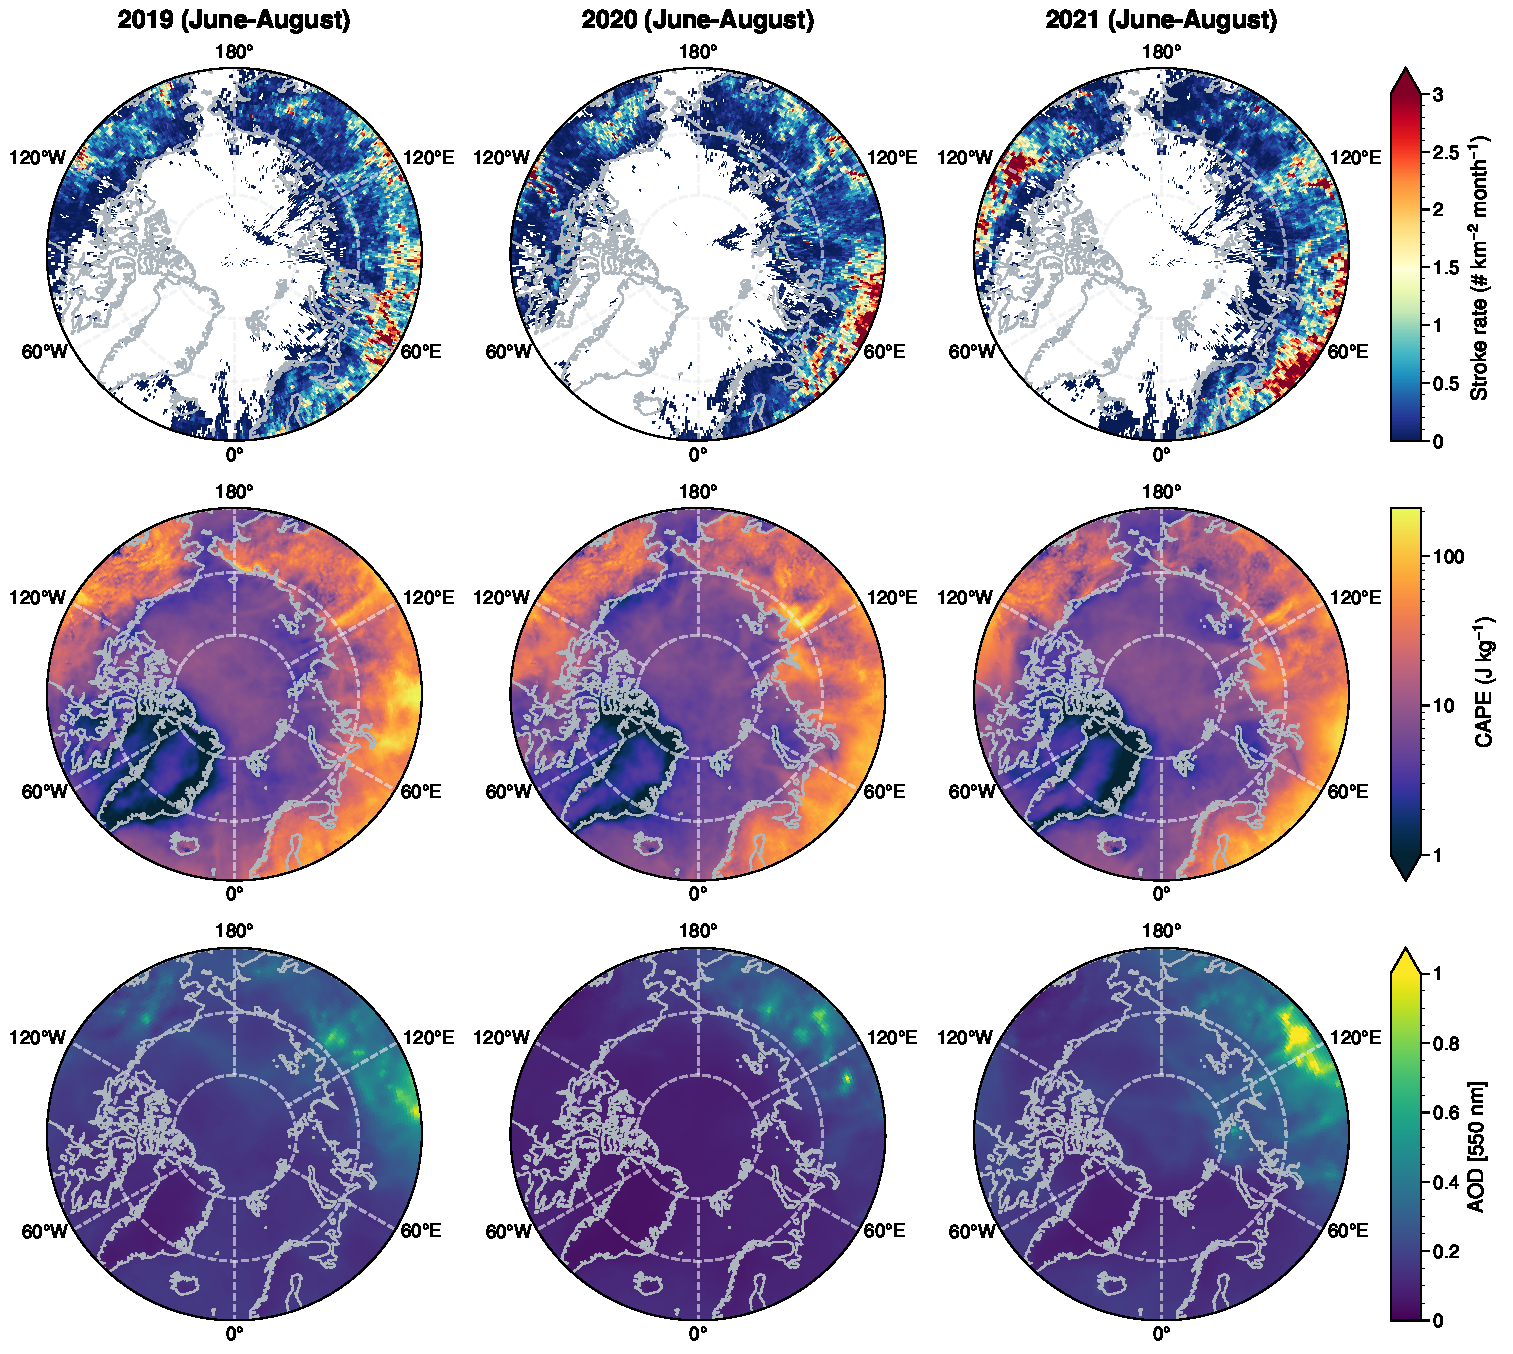
\includegraphics[width=16cm]{./figures/arctic_cape_aod.pdf}
\caption{
2019至2021年夏季(6--8月)平均 GLD360 闪击频率、对流有效位能(CAPE,来自 ERA5)和气溶胶光学厚度(550 nm 处的 AOD,来自 MERRA-2)。\\
Figure \ref{fig:arctic_cape_aod}.
Mean GLD360 lightning stroke rate, convective available potential energy (CAPE, from ERA5), and aerosol optical depth (AOD at 550 nm, from MERRA-2) over June--August of 2019–-2021.
}
\label{fig:arctic_cape_aod}
\end{figure}


\begin{figure}[htbp]
\centering
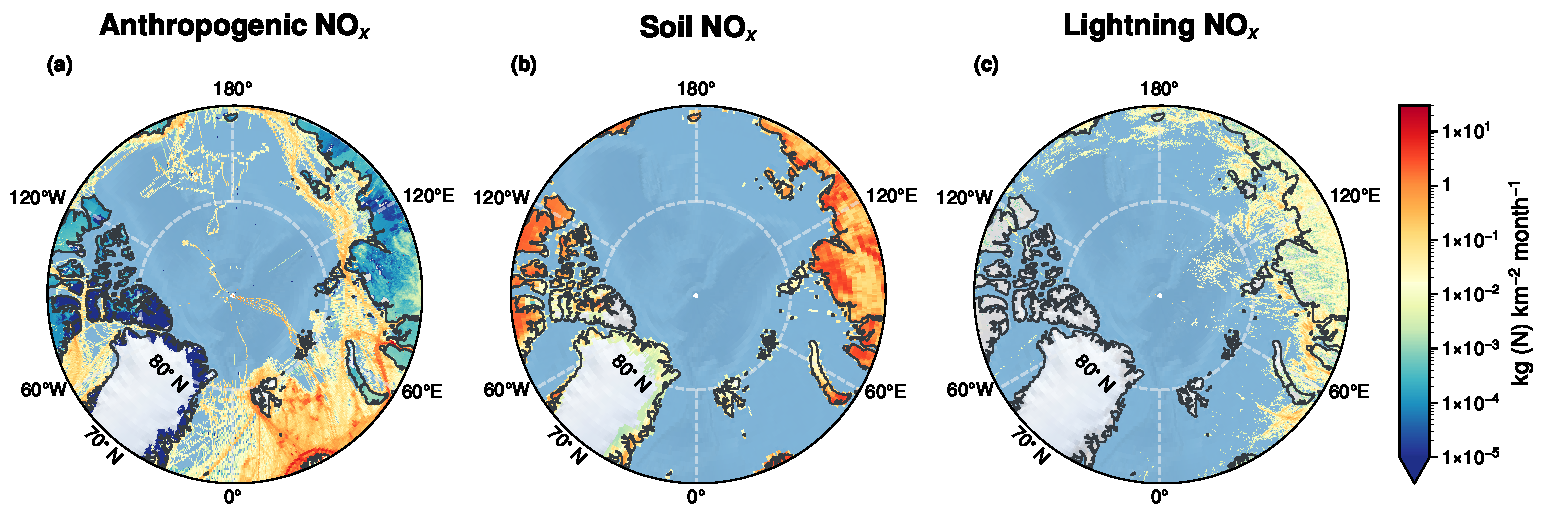
\includegraphics[width=15cm]{./figures/arctic_emission_comp.pdf}
\caption{
北极地区6--8月的NO$_x$月排放量
(a) 人为排放(包括船舶排放),(b) 土壤排放,
(c) 船舶排放。
闪电 NO$_x$ 排放是 2019 年至 2021 年的平均值。
其他排放来自哥白尼大气监测服务 (CAMS) 2018 年全球排放清单。\\
Figure \ref{fig:arctic_emission_comp}. Monthly NO$_x$ emissions in the Arctic from June to August.
(a) Anthropogenic emissions including ship emissions, (b) Soil emissions, and (c) Lightning emissions.
The lightning NO$_x$ emissions are the mean values from 2019 to 2021, while the other emissions are from the 2018 Copernicus Atmosphere Monitoring Service (CAMS) global emission inventories.
}
\label{fig:arctic_emission_comp}
\end{figure}


图 \ref{fig:arctic_no2_comp}a 显示了 2019--2021 年 6 月至 8 月 TROPOMI 在北极观测到的平均 NO$_2$ 浓度。
虽然从背景中无法看出平均LNO$_2$,但在城市、工业和野火地区仍然可以观察到 NO$_2$ 的增强。
例如,可以清楚地观察到与阿拉斯加、挪威和俄罗斯的采矿作业相关的 NO$_2$ (17 $\pm$ 2 $\mu$mol m$^{-2}$)。
其他例子是与加拿大北极麦肯齐谷、北阿拉斯加普拉德霍湾/库帕鲁克和俄罗斯亚马尔天然气管道/乌连戈气田相关的石油和天然气活动 \citep{VanDerA.2020}。
ß格陵兰海岸沿线的 NO$_2$ 峰值可能是与复杂地形反演相关的错误信号\citep{Hachmeister.2022}。
与 NO$_2$ 污染相反,70$^{\circ}$ N 以北的 TROPOMI 观测显示低浓度的背景 NO$_2$(4.35 $\pm$ 1.26 $\mu$mol m$^{-2}$),
比 60$^{\circ}$ N 和 65$^{\circ}$ N 之间的平均 NO$_2$ 少 45\%。

通过将每个个例中LNO$_2$柱密度的最大值(61 $\pm$ 50 $\mu$mol m$^{-2}$) 与北极地区典型的人为和野火 NO$_2$ 进行比较,
我们发现 LNO$_2$ 的柱密度为其他源的3倍,尽管排放的时间尺度是小时数量级(图 \ref{fig:arctic_no2_comp}b)。
其中发生在拉普捷夫海(Laptev Sea)上空的深层对流(图\ref{fig:arctic_large_lno2}),
其LNO$_2$最大值 为 246 $\mu$mol m$^{-2}$,是美国最高 NO$_2$ 柱密度相当(234 $\mu$mol m$^{-2}$,\citet{Goldberg.2021a})。
考虑到LNO$_2$在短时间内的巨大贡献,因此计算北极地区LNO$_2$的排放很重要。

\begin{figure}[!htbp]
\centering
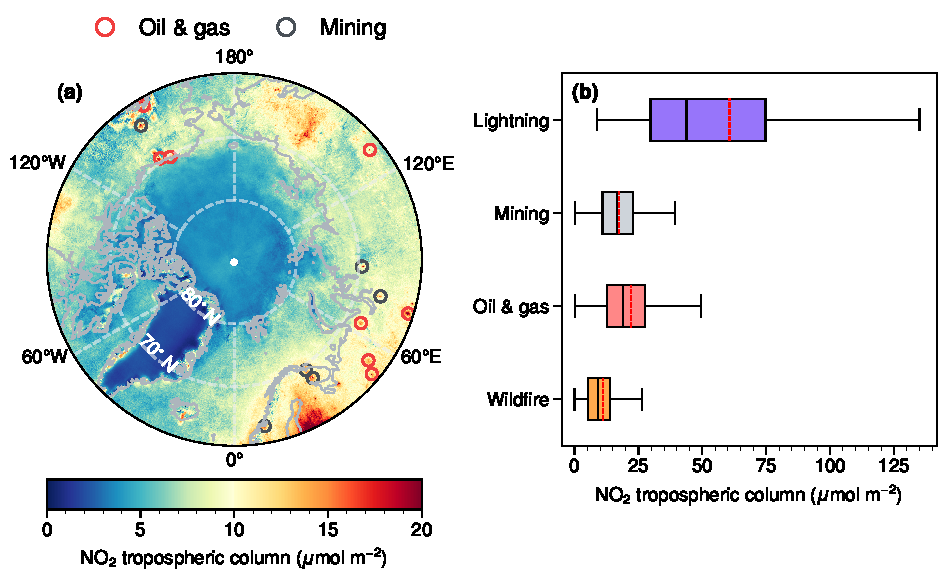
\includegraphics[width=15cm]{./figures/arctic_no2_comp.pdf}
\caption{
(a) 2019 年 8 月至 2021 年 6 月当地下午TROPOMI测的的对流层 NO$_2$ 平均柱密度(4 km $\times$ 4 km)。
采矿和石油 \& 加油站是面板(a)中显示的灰色和红色圆圈。
(b) NO$_2$ 四种来源的比较:闪电、采矿、石油\&天然气和野火。
其中闪电LNO$_2$的浓度为每次闪电个例的所有像素上NO$_2$的最大值,而野火、采矿和石油 \& 天然气的浓度是典型位置的每日最大 NO$_2$ 值。
框内的线分别是中值(黑色)和平均值(红色)。
下边界和上边界分别是第 25 和第 75 个百分位数。
上下误差线分别是第 10 和第 90 个百分位数,\\
Figure \ref{fig:arctic_no2_comp}(a) Mean 4 km $\times$ 4 km TROPOMI tropospheric NO$_2$ column density in the local afternoon during June--August of 2019--2021.
The mining and oil \& gas stations are gray and red circles shown in panel (a).
(b) Comparisons of NO$_2$ among four sources: lightning, mining, oil \& gas, and wildfire.
The bar of lightning represents the maximum NO$_2$ values over pixels of each lightning case.
The wildfire, mining, and oil \& gas bars are the daily maximum NO$_2$ values over typical locations.
The lines inside box are median (black) and mean (red) values, respectively.
Lower and upper box boundaries are 25th and 75th percentiles, respectively.
Lower and upper error lines are 10th and 90th percentiles, respectively,
}
\label{fig:arctic_no2_comp}
\end{figure}

\begin{figure}[!htbp]
\centering
\includegraphics[width=18cm]{./figures/arctic_large_lno2.pdf}
\caption{
(a) 在 500 hPa气压层水平传输的包含闪电 NO$_2$ 的空气块。
(b) TROPOMI 检测到的 NO$_2$ 对流层柱密度。
(c) TROPOMI 检测到的云压。\\
(a) Transported air parcels containing lightning NO$_2$ at 500 hPa pressure level.
(b) The TROPOMI-detected NO$_2$ tropospheric columns.
(c) The TROPOMI-detected cloud pressures.
}
\label{fig:arctic_large_lno2}
\end{figure}


\section{污染地区(中国及美国大陆)}

\subsection{模式设置} \label{sec:model_settings}

使用的WRF-Chem版本为3.5.1,水平网格大小为12 km $\times$ 12 km (图\ref{fig:us_domain}a),垂直层数为29层,时间步长为72 s。
气象条件的初始场和边界场为时间分辨率3小时的北美区域再分析(NARR)数据集,每3小时应用一次边界条件和四维数据分析(FDDA)逼近,
其中温度、水汽和水平风以0.0003 s$^{-1}$ 的系数逼近\citep{Laughner.2017}。
微物理过程采用Lin方案\citep{Lin.1983},积云参数化为Grell 3D方案\citep{Grell.1993a,Grell.2002a},长波辐射采用RRTM方案\citep{Iacono.2008},短波辐射采用Goddard方案,陆面过程使用Noah陆面模式\citep{Koren.1999},边界层采用YSU方案\citep{Hong.2006}。
闪电参数化采用基于对流参数化的中性浮力水平\citep{Pickering.1992},云闪与地闪的比例基于\citet{Boccippio.2001}.

采用臭氧和相关化学示踪剂模型第4版(MOZART-4;\citet{Emmons.2010})的输出场作为化学的初始场和边界场。
人为排放由2011年美国国家排放清单(NEI)驱动,并根据环境保护署年度总排放量,按模拟的年份进行调整\citep{EPA.2015}。
生物排放使用MEGAN源,化学机制是区域大气化学机制第2版(RACM2;\citet{Goliff.2013}),并由\citet{Browne.2014}和\citet{Schwantes.2015}进行了更新。
此外,LNO$_x$参数化采用每次闪电产生200 mol NO,调整因子为1,以下简称“1$\times$200 mol NO per flash”)。
基于\citet{Ott.2010}的双峰型闪电NO(LNO)廓线\citep{Laughner.2017}被用作 WRF-Chem中LNO的垂直分布,而LNO和LNO$_2$廓线是指有和没有闪电的模拟之间垂直廓线的差异。


\begin{figure}[htbp]
\centering
\includegraphics[width=11cm]{./figures/us_domain.png}
\caption{WRF-Chem 模拟区域和地形高度 (m),网格数为 350 $\times$ 290,水平分辨率为 12 km \\
Figure \ref{fig:us_domain}. Domain and terrain height (m) of the WRF-Chem simulation with 350 x 290 grid cells and a horizontal resolution of 12 km.}
\label{fig:us_domain}
\end{figure}


\subsection{闪电氮氧化物的反演} \label{subsec:retrieval_polluted}

首先我们使用恒定值网格化法,将公式(\ref{eq:AMF_LNO2})所得的LNO$_x$垂直柱密度(V$_{\textrm{NO$_x$}}$)分配至0.05$^{\circ}$ $\times$ 0.05$^{\circ}$网格\citep{Kuhlmann.2014}。
接着在 1$^{\circ}$ $\times$ 1$^{\circ}$的网格中进行分析,要求每个网格至少有50个有效的0.05$^{\circ}$ $\times$ 0.05$^{\circ}$网格数据,从而最小化噪点数据。
具体LNO$_x$的主要计算步骤如下。

云辐射分数(CRF,CRF $\geq$ 70\%,CRF $\geq$ 90\%,CRF = 100\%)和 云压(CP,CP $\leq$ 650 hPa)是OMI像素是否包含深对流云的判断标准\citep{Ziemke.2009,Choi.2014,Pickering.2016}。
不同CRF对LNO$_x$产品的影响将在\ref{subsec:retrieval_polluted}节探讨。
此外,我们将另一个云分数 (CF) 标准应用于 WRF-Chem 的模拟结果,以确保对流被成功模拟。
具体而言,CF是由 Xu-Randall 方法计算的 350--400 hPa 之间的最大云分数\citep{Xu.1996,Strode.2017}。
选择350--400 hPa的大气层,可避免模拟高云中的偏差。
我们选择\citet{Strode.2017}建议的 CF $\geq$ 40\%来判断模拟所处的网格是多云或晴空。

除了云特性之外,OMI能探测到新生LNO$_x$的另一条件为一段时间内有足够的闪电或闪击。
其中,时间窗口 (t$_{window}$) 是 OMI 过境之前的时间段。
\citet{Lapierre.2020}利用1$^{\circ}$ $\times$ 1$^{\circ}$网格的对角线长度和OMI过境时美国大陆上空500--100 hPa的平均风速计算得到t$_{window}$为2.4 h。
同时,\citet{Lapierre.2020}定义在t$_{window}$时间段内,至少发生2400次闪电或8160次闪击的网格才能提供足够的LNO$_x$给OMI探测。
\citet{Bucsela.2019}的研究表明,低频率的闪电具有更高的LNO$_x$产率(PE),而该段数据在\citet{Lapierre.2020}研究中被剔除。
通过比较使用每个网格至少2400次闪电和至少1次闪电的标准所得结果,我们也得到相同的结论(图\ref{fig:us_flash_threshold})。
由于我们的研究重点是开发一种新的空气质量转换因子(AMF),并将计算结果与使用类似闪电阈值的其他产品进行比较\citep{Pickering.2016,Lapierre.2020},
因此我们接下来使用相同的至少2400次闪电标准来进行结果分析。


\begin{figure}[htbp]
    \includegraphics[width=15cm]{./figures/us_flash_threshold.pdf}
    \caption{
    (a) 每日 LNO$_x$ 产率与 ENTLN 总闪的关系,筛选条件为CRF $\geq$ 90\% 且1$^{\circ}$ $\times$ 1$^{\circ}$网格中至少有1次闪电。
     (b) 与 (a) 相同,但针对闪击。\\
    Figure \ref{fig:us_flash_threshold}. (a) Daily LNO$_\textrm{x}$ production efficiencies versus ENTLN total flashes data, with CRF $\geq$ 90\% and a flash threshold of 1 flash box$^{-1}$.
    (b) Same as (a) but for strokes.}
    \label{fig:us_flash_threshold}
\end{figure}


为确保WRF-Chem成功模拟闪电并考虑到闪电参数化的不确定性,我们将每个1$^{\circ}$ $\times$ 1$^{\circ}$网格模拟的总闪电(TL)阈值设置为1000,该阈值低于ENTLN闪电观测使用的阈值。
针对除LNO$_2$之外的其他NO$_2$源,我们定义了模拟的云上闪电NO$_2$柱密度(LNO$_2$Vis)与云上NO$_2$柱密度(NO$_2$Vis)之比,来判断OMI是否可以检测到足够的LNO$_2$。
该比率$\geq$50\%表明云层上方超过一半的NO$_x$具有LNO$_x$源。
此外,还需考虑氧化有关的NO$_2$寿命。
\citet{Nault.2017}的研究表明NO$_2$在对流附近的寿命($\tau$)为$\approx$3 h,故NO$_2$的初始值可由方程式(\ref{eq:inition})求解。

\begin{equation} \label{eq:inition}
NO_2(0) = NO_2(OMI) \times e^{0.5t/\tau}
\end{equation}

其中$NO_2(0)$是在时间 t=0 排放的NO$_2$摩尔数,$NO_2(OMI)$是在 OMI 过境时间测得的NO$_2$摩尔数,
0.5t是穿过网格的时间,即1.2 h,(假设闪电出现在每个1$^{\circ}$ $\times$ 1$^{\circ}$网格的中心)。
每个网格的V$_\textrm{LNO$_x$}$为网格中所有0.05$^{\circ}$ $\times$ 0.05$^{\circ}$像素的V$_\textrm{LNO$_x$}$平均值,
然后乘以网格的面积得到LNO$_x$摩尔数。

最后,有两种方法可用于估算季节性平均LNO$_2$每闪电、LNO$_x$每闪电、LNO$_x$每闪击和 LNO$_x$每闪击:

(1)求和法,将LNO$_x$的总和除以5--8月中每个1$^{\circ}$ $\times$ 1$^{\circ}$网格里发生的闪电或闪击总数;

(2)线性回归方法,将线性回归应用于LNO$_x$和每日闪电或闪击的平均值。

% \subsection{适合反演闪电氮氧化物的条件} \label{subsec:criteria}

根据以上条件,我们定义了六种不同的筛选条件组合(表),并使用线性回归方法(表)应用于原始数据。

\begin{table*}[htbp]
\scriptsize
\caption{本研究中使用的标准的缩写定义\\Table \ref{table:Abbreviations}Definitions of the abbreviations for the criteria used in this study.}
\begin{tabular}{ll}
\hline
\textbf{缩写} & \textbf{全称 [来源]} \\
\hline
CRF                             & Cloud radiance fraction [OMI] \\
CP                              & Cloud optical pressure [OMI] \\
CF                              & Cloud fraction [WRF-Chem] \\
TL                              & Total lightning flashes [WRF-Chem] \\
ratio                           & modeled LNO$_2$Vis / modeled NO$_2$Vis [WRF-Chem] \\
CRF$\alpha$\_ENTLN                    & CRF $\geq$ $\alpha$ + ENTLN flashes(strokes) $\geq$ 2400(8160) [ENTLN]\\
CRF$\alpha$\_CF40\_ENTLN              & CRF $\geq$ $\alpha$ + ENTLN flashes(strokes) $\geq$ 2400(8160) + CF $\geq$ 40\% \\
CRF$\alpha$\_ENTLN\_TL1000            & CRF $\geq$ $\alpha$ + ENTLN flashes(strokes) $\geq$ 2400(8160) + TL $\geq$ 1000 \\
CRF$\alpha$\_CF40\_ENTLN\_TL1000      & CRF $\geq$ $\alpha$ + ENTLN flashes(strokes) $\geq$ 2400(8160) + CF $\geq$ 40\% + TL $\geq$ 1000 \\
CRF$\alpha$\_ENTLN\_TL1000\_ratio50   & CRF $\geq$ $\alpha$ + ENTLN flashes(strokes) $\geq$ 2400(8160) + TL $\geq$ 1000 + ratio $\geq$ 50\% \\
CRF$\alpha$\_CF40\_ENTLN\_TL1000\_ratio50 & CRF $\geq$ $\alpha$ + ENTLN flashes(strokes) $\geq$ 2400(8160) + CF $\geq$ 40\% + TL $\geq$ 1000 + ratio $\geq$ 50\% \\
CRF$\alpha$\_ENTLN1(3.4)\_TL1\_ratio50    & CRF $\geq$ $\alpha$ + ENTLN flashes(strokes) $\geq$ 1(3.4) + TL $\geq$ 1 + ratio $\geq$ 50\% \\
\hline
\multicolumn{2}{l}{$^{*}$$\alpha$有三种选择:70\%、90\%以及100\%} \\
\multicolumn{2}{l}{$^{*}$$\alpha$ has three options: 70\%, 90\% and 100\%}
\end{tabular}
\label{table:Abbreviations}
\end{table*}


\begin{table*}[htbp]
\scriptsize
\caption{根据表\ref{table:Abbreviations}中的定义得到的LNO$_\textrm{x}$产率\\Table \ref{table:conditions} LNO$_\textrm{x}$ production efficiencies for different combinations of criteria defined in Table \ref{table:Abbreviations}.}
\begin{tabular}{lccccc}
\hline
\textbf{条件$^1$} & \textbf{ENTLN类型$^2$} & \textbf{LNO$_\textrm{x}$/flash or LNO$_\textrm{x}$/stroke} & \textbf{R值} & \textbf{截距 (10$^{6}$mol)} & \textbf{天数$^3$} \\
\hline
CRF90\_ENTLN                        & Flash  & 52.1 $\pm$ 51.1 & 0.20 & 0.21  & 99 \\
CRF90\_CF40\_ENTLN                  & Flash  & 84.2 $\pm$ 31.5 & 0.54 & -0.04 & 70 \\
CRF90\_ENTLN\_TL1000                & Flash  & 61.9 $\pm$ 49.1 & 0.27 & 0.33  & 83 \\
CRF90\_CF40\_ENTLN\_TL1000          & Flash  & 63.4 $\pm$ 52.9 & 0.38 & 0.26  & 38 \\
CRF90\_ENTLN\_TL1000\_ratio50       & Flash  & 54.5 $\pm$ 48.1 & 0.25 & 0.39  & 81 \\
CRF90\_CF40\_ENTLN\_TL1000\_ratio50 & Flash  & 90.0 $\pm$ 65.0 & 0.46 & 0.15  & 32 \\
CRF90\_ENTLN                        & Stroke & 6.7 $\pm$ 4.1 & 0.31 & 0.23  & 102 \\
CRF90\_CF40\_ENTLN                  & Stroke & 10.3 $\pm$ 3.6 & 0.55 & 0.08 & 79 \\
CRF90\_ENTLN\_TL1000                & Stroke & 7.5 $\pm$ 5.1 & 0.29 & 0.38  & 94 \\
CRF90\_CF40\_ENTLN\_TL1000          & Stroke & 8.6 $\pm$ 6.2 & 0.39 & 0.27  & 46 \\
CRF90\_ENTLN\_TL1000\_ratio50       & Stroke & 7.0 $\pm$ 4.8 & 0.29 & 0.42  & 93 \\
CRF90\_CF40\_ENTLN\_TL1000\_ratio50 & Stroke & 8.9 $\pm$ 7.0 & 0.39 & 0.31  & 40 \\
\hline
\multicolumn{6}{l}{$^1$定义见表\ref{table:Abbreviations}。}\\
\multicolumn{6}{l}{$^2$ENTLN阈值为OMI过境前2.4小时内,1$^{\circ}$ $\times$ 1$^{\circ}$网格中闪电至少2400次和闪击至少8160次。}\\
\multicolumn{6}{l}{$^3$2014年5--8月中有效的天数。} \\
\multicolumn{6}{l}{$^1$These conditions are defined in Table \ref{table:Abbreviations}.} \\
\multicolumn{6}{l}{$^2$The thresholds of ENTLN data are 2400 flashes box$^{-1}$ and 8160 strokes box$^{-1}$ during the period of 2.4 h before OMI overpass time.} \\
\multicolumn{6}{l}{$^3$The number of valid days with specific criteria in MJJA 2014.}
\label{table:conditions}
\end{tabular}
\end{table*}


在CRF90\_ENTLN条件下,有效闪电(闪击)数据对应共有99(102)天。
以闪电类ENTLN数据为例,在 CRF90\_ENTLN\_TL1000\_ratio50 条件下,有效天数从 99 减少至 81,而LNO$_x$产率从 52.1$\pm$51.1 mol每闪电增加到 54.5$\pm$48.1 mol每闪电。
该结果与 CRF90\_ENTLN\_TL1000 条件下所得的结果几乎相同。
尽管这表明TL筛选条件已足够严格,但最好包括云上LNO$_2$占比的筛选条件,以防不同的AMF方法中存在一些例外情况。
由于 CF $\geq$ 40\% 会导致有效数据和产率急剧下降,因此我们仅仅使用 CRF 对数据进行筛选。
最后,我们选择至少2400次闪电或至少8160次闪击,TL $\geq$ 1000 和云上LNO$_2$占比 $\geq$ 50\% 作为阈值,来探索三种不同 CRF 条件(CRF $\geq$ 70\%、CRF $\geq$ 90\% 和 CRF = 100\%)对 LNO$_x$ 估算产生的影响(表\ref{table:CRFs})。
当CRF 标准从 70\% 增加到 90\% 和 100\%时,针对闪电类型的LNO$_x$产率 从35.7$\pm$36.8 mol每闪电增加到 54.5$\pm$48.1 mol每闪电,然后再降低到20.8$\pm$37.4 mol每闪电,而针对闪击类型的LNO$_x$产率从4.1$\pm$3.9 mol每闪击提高到 7.0$\pm$4.8 mol每闪击,然后再次下降到2.6$\pm$4.0 mol每闪击(表\ref{table:CRFs})。
当 CRF 从 90\% 增加到 100\% 时LNO$_x$ PE 降低,这是因为闪电密度较高而 LNO$_x$ 较少。
CRF 从 70\% 增加到 90\% 引起的 LNO$_x$ PE 增加与\citet{Pickering.2016}的结果相反。
这是由于我们的方法中考虑了从边界层传输的 NO$_2$ 污染的影响。
虽然在 CRF > 70\% 的地区经常观察到 NO$_x$ 增强\citet{Pickering.2016},但考虑到中低浓度 NO$_2$ 的污染并与\citet{Pickering.2016}和\citet{Lapierre.2020}的结果进行比较,以下分析将基于 CRF $\geq$ 90\% 标准进行讨论分析。

\begin{table*}[htbp]
\scriptsize
\caption{在相同ENTLN阈值,TL $\geq$ 1000 和云上LNO$_2$占比 $\geq$ 50\%的条件下,不同云辐射分数阈值对应的LNO$_\textrm{x}$产率 \\ LNO$_\textrm{x}$ production efficiencies for different thresholds of CRF with coincident ENTLN data, TL $\geq$ 1000 and ratio $\geq$ 50\%.}
\begin{tabular}{cccccc}
\hline
\textbf{云辐射分数 (\%)} & \textbf{ENTLN类型$^1$} & \textbf{LNO$_\textrm{x}$每闪电 or LNO$_\textrm{x}$每闪击} & \textbf{R值} & \textbf{截距 (10$^{5}$mol)} & \textbf{天数$^2$} \\
\hline
70  & 闪电  & 35.7  $\pm$ 36.8 & 0.21 & 4.91 & 85 \\
90  & 闪电  & 54.5  $\pm$ 48.1 & 0.25 & 3.90 & 81 \\
100 & 闪电  & 20.8  $\pm$ 37.4 & 0.13 & 5.67 & 71 \\
70  & 闪击 & 4.1   $\pm$ 3.9  & 0.21 & 5.16 & 96 \\
90  & 闪击 & 7.0   $\pm$ 4.8  & 0.29 & 4.16 & 93 \\
100 & 闪击 & 2.6   $\pm$ 4.0  & 0.14 & 5.41 & 82 \\
\hline
\multicolumn{6}{l}{$^1$ENTLN阈值为 OMI f过境前 2.4 小时内每个网格闪电至少 2400 次 或 闪击至少8160 次。}\\
\multicolumn{6}{l}{$^2$2014年5--8月对应筛选条件下有效天数。} \\
\multicolumn{6}{l}{$^1$The thresholds of ENTLN data are 2400 flashes box$^{-1}$ and 8160 strokes box$^{-1}$ during the period of 2.4 h before OMI overpass time.}\\
\multicolumn{6}{l}{$^2$The number of valid days with specific criteria in MJJA 2014.}
\end{tabular}
\label{table:CRFs}
\end{table*}

\subsection{闪电氮氧化物的产率}
% \subsection{基于不同反演方法的结果对比}

\citet{Lapierre.2020}基于 BEHR NO$_2$ 产品得出 LNO$_2$ 产量,
为了使本研究的结果与\citet{Pickering.2016}和\citet{Lapierre.2020}的结果具有可比性,我们选择 NO$_2$  而不是 NO$_x$  来计算每次闪电的产量(产率,PE)。
在图\ref{fig:us_pe_timeseries}中,根据 CRF $\geq$ 90\% 和每 2.4 h 2400次闪电的阈值,绘制了2014年5--8月美国大陆每天 NO$_2$Vis、LNO$_2$Vis、LNO$_2$ 和 LNO$_2$Clean 产率的时间序列图。
其中,LNO$_2$ PE 大多在 20 至 80 mol每闪电的范围内,LNO$_2$Vis PE 小于 LNO$_2$ PE,因为后者在云层下含有 LNO$_2$。
\citet{Pickering.2016}的GMI模拟结果表明,25\%--30\%的LNO$_x$柱密度位于 云压(CP)以下,而我们的 WRF-Chem 模拟结果显示该比例为 56$\pm$20\%。
云属性对 LNO$_x$ PE 的影响将在第\ref{sec:uncertainty}节中进行更详细地讨论。
总体而言,估算得到的每日PE顺序为LNO$_2$Clean > LNO$_2$ > NO$_2$Vis > LNO$_2$Vis。
通过NO$_2$Vis 和 LNO$_2$Vis 估算得到的PE之间的差异($\Delta$PE)表明有一定量的背景 NO$_2$ 存在于云层之上。
总体而言,该 $\Delta$PE 的趋势与 NO$_2$Vis 和 LNO$_2$Clean 之间的$\Delta$PE 一致。
当区域污染严重时(NO$_2$Vis 和 LNO$_2$Vis 之间的 $\Delta$PE > 200\%),基于 NO$_2$Vis 和 LNO$_2$Clean 的 PE 被显著高估。
换言之,NO$_2$Vis 和 LNO$_2$Clean 对背景 NO$_2$ 更为敏感。
且在高污染地区,NO$_2$Vis 的高估程度大于 LNO$_2$Clean,而在其他大多数地区通常相反。

\begin{figure}[htbp]
\centering
\includegraphics[width=12cm]{./figures/us_pe_timeseries.pdf}
\caption{(上图)NO$_2$Vis、LNO$_2$Vis、LNO$_2$ 和 LNO$_2$Clean产率的时间序列(2014年5--8月美国大陆),筛选条件为CRF $\geq$ 90\% 和每 2.4 小时 至少2400 次闪电。
(下图)在CRF$\geq$ 90\%的条件下,NO$_2$Vis 和 LNO$_2$Vis 之间百分比差异以及 NO$_2$Vis 和 LNO$_2$Clean 之间百分比差异的时间序列。
8 月 23 日黑点的值(未显示)为 1958\%。\\
Figure \ref{fig:us_pe_timeseries}. (top) Time series of NO$_2$Vis, LNO$_2$Vis, LNO$_2$ and LNO$_2$Clean production per day over the CONUS for MJJA 2014 with CRF $\geq$ 90\% and a flash threshold of 2400 flashes per 2.4 h.
(bottom) Time series of the percent differences between NO$_2$Vis and LNO$_2$Vis and the percent differences between NO$_2$Vis and LNO$_2$Clean with CRF $\geq$ 90\%.
The value of black dot on August 23 (not shown) is 1958\%.}
\label{fig:us_pe_timeseries}
\end{figure}

如图\ref{fig:us_pe_linear}所示,ENTLN 数据与 NO$_2$Vis、LNO$_2$Vis、LNO$_2$ 和 LNO$_2$Clean的线性回归,其筛选条件与图 \ref{fig:us_pe_timeseries} 相同。
LNO$_2$Clean PE为 25.2$\pm$22.3 mol NO$_2$ 每闪电,相关系数为 0.25 和 2.3$\pm$2.1 mol NO$_2$每闪击,相关系数为 0.22。
如图\ref{fig:us_pe_timeseries}所示,NO$_2$Vis PE 和 LNO$_2$Clean PE 之间的正百分比差异发生的频率远低于负差异的发生频率。
因此,NO$_2$Vis PE(17.1$\pm$17.2 mol NO$_2$ 每闪电和0.4$\pm$1.0 mol NO$_2$ 每闪击)小于使用线性回归方法得到的 LNO$_2$Clean PE。

\begin{figure}[t]
    \includegraphics[width=15cm]{./figures/us_pe_linear.pdf}
    \caption{(a) 每日 NO$_2$Vis、LNO$_2$Vis、LNO$_2$ 和 LNO$_2$Clean 与 ENTLN 总闪的关系。
    (b) 与 (a) 相同,但针对闪击数据。
    (c) 每日 LNO$_x$Vis 和 LNO$_x$ 与总闪的关系。
    (d) 与 (c) 相同,但针对闪击数据。\\
    Figure \ref{fig:us_pe_linear}. (a) Daily NO$_2$Vis, LNO$_2$Vis, LNO$_2$ and LNO$_2$Clean versus ENTLN total flashes data.
    (b) Same as (a) but for strokes. (c) Daily LNO$_x$Vis and LNO$_x$ versus total flashes. (d) Same as (c) but for strokes.}
    \label{fig:us_pe_linear}
\end{figure}

为了将我们的结果与\citet{Lapierre.2020}的结果进行比较,
我们从筛选条件中取出CP $\leq$ 650 hPa、TL $\geq$ 1000 和 ratio $\geq$ 50 \% 的条件。
但是,我们得到的NO$_2$Vis(3.8$\pm$0.5 mol每闪击)仍大于\citet{Lapierre.2020}的1.6$\pm$0.1 mol每闪击。
这可能是由两者使用不同版本的伯克利高分辨率(BEHR)算法引起的,\citet{Lapierre.2020}使用的是BEHR v3.0A,我们的算法基于BEHR v3.0B \citep{Laughner.2019a}。
两个版本中S$_{\textrm{NO$_2$}}$均来自于NASA标准产品v3,BEHR v3.0B 的主要改进如下:

(1)使用最接近 OMI 过境时间的廓线,而不是 OMI 过境之前的最后一个时刻的廓线;

(2)AMF 使用可变的对流层顶高度,而不是固定的200 hPa 对流层顶;

(3)根据\citet{Zhou.2009}的方法计算地表气压。

详细的更新日志见\url{https://github.com/CohenBerkeleyLab/BEHR-core/blob/master/Documentation/Changelog.txt}。
此外,\citet{Lapierre.2020}使用了月平均NO$_2$廓线,而我们的研究使用了日廓线,并且我们将WRF-Chem 输出的间隔调整为 30 min,
这比BEHR 每日产品(1 h)输出间隔更短,但 AMF 可能会受到不同 NO$_2$ 剖面的影响。
鉴于这些因素,我们在所得数据的基础上来比较不同的方法,以尽量减少这些影响。

同时,LNO$_2$ PE(18.7$\pm$18.1 mol每闪电,2.1$\pm$1.8 mol每闪击)介于 LNO$_2$Clean PE 和 NO$_2$Vis PE 之间,与图 \ref{fig:us_pe_timeseries} 中的日结果一致。
此外,基于每日LNO$_x$ PE 求和值的线性回归结果为114.8$\pm$18.2 mol每闪电(或17.8$\pm$2.9 mol每闪击),该结果大于\citet{Pickering.2016}的91 mol每闪电。
这一差异可能是由地理位置、闪电数据和化学模型所共同导致的。

在 CRF $\geq$ 90\% 下,LNO$_2$ PE 的平均值和标准差为 46.2$\pm$35.1 mol 每闪电和 9.9$\pm$8.1 mol 每闪电,
而 LNO$_x$ PE 为 125.6$\pm$95.9 mol 每闪电和 26.7$\pm$21.6 mol 每闪电(图\ref{fig:us_pe_sum})。
美国东南部的 LNO$_2$ PE 和 LNO$_x$ PE 均较高(由图\ref{fig:us_pe_sum}中的红框表示,25--37$^{\circ}$ N,75--95$^{\circ}$ W),这与\citet{Lapierre.2020} 和 \citet{Bucsela.2019}的研究结果相一致。
而与图\ref{fig:us_pe_timeseries}相比,图\ref{fig:us_delta}(a)和(b)显示NO$_2$Vis PE 和 LNO$_2$Vis PE 之间的一些较大差异,这与我们对污染区域的预期一致。
同时,LNO$_2$ PE 和 NO$_2$Vis PE 之间的差异取决于背景 NO$_2$、上升气流的强度和廓线分布。
负差异是由上升气流携带的背景 NO$_2$ 引起的,而云下 LNO$_2$ 的部分导致 LNO$_2$ PE 高于 NO$_2$Vis PE(图\ref{fig:us_delta}(c))。
图\ref{fig:us_delta}(d) 显示 LNO$_2$Vis 与 LNO$_2$占比为 10\%--80\%。
这可能是由云层的高度和 LNO$_2$ 的廓线造成的。
如果CP在300 hPa附近,由于云层的覆盖,该比值将更小。
因此,需要更好地了解LNO$_2$ 廓线和 云下的LNO$_x$。


\begin{figure}[htbp]
\centering
\includegraphics[width=13cm]{./figures/us_pe_sum.png}
\caption{(a) 和 (c) 在CRF $\geq$ 90\%条件下,2014年5--8月 1$^{\circ}$ $\times$ 1$^{\circ}$ LNO$_\textrm{x}$ 和LNO$_\textrm{2}$的平均产率分布图。
     (b) 和 (d) 与 (a) 和 (c) 相同,但针对闪击数据。美国东南部由红框表示。\\
     Figure \ref{fig:us_pe_sum}. (a) and (c) Maps of 1$^{\circ}$ $\times$ 1$^{\circ}$ gridded values of mean LNO$_\textrm{x}$
    and LNO$_\textrm{2}$ production per flash with CRF $\geq$ 90\% for MJJA 2014.
    (b) and (d) Same as (a) and (c) except for strokes.
    The southeastern US is denoted by the red box in panels a--d.
}
\label{fig:us_pe_sum}
\end{figure}

\begin{figure}[t]
\centering
\includegraphics[width=13cm]{./figures/us_delta.png}
\caption{(a) 2014年5--8月  平均对流层NO$_\textrm{2}$柱浓度。
污染城市用星星表示:兰辛、新奥尔良和奥兰多,而清洁城市用三角形表示:休伦、查尔斯镇和塔伯勒。
(b) 在CRF $\geq$ 90\%条件下,NO$_\textrm{2}$Vis 和 LNO$_\textrm{2}$Vis平均产率的差异。
(c) 与 (b) 相同,但为 LNO$_\textrm{2}$ 和 NO$_\textrm{2}$Vis 之间的差异。
(d) LNO$_\textrm{2}$Vis 与 LNO$_\textrm{2}$ 的比例。\\
Figure \ref{fig:us_delta}.
(a) Mean (MJJA 2014) NO$_\textrm{2}$ tropospheric column.
Polluted cities are denoted by stars: Lansing, New Orleans and Orlando while clean cities are denoted by triangles: Huron, Charles Town and Tarboro.
(b) The differences of the estimated mean production efficiency between NO$_\textrm{2}$Vis and LNO$_\textrm{2}$Vis with CRF $\geq$ 90\%.
(c) The same differences as (b) but between LNO$_\textrm{2}$ and NO$_\textrm{2}$Vis.
(d) The ratio of LNO$_\textrm{2}$Vis to LNO$_\textrm{2}$.
}
\label{fig:us_delta}
\end{figure}

\subsection{反演的影响因素及不确定性分析} \label{sec:uncertainty}

鉴于图\ref{fig:us_delta}表明我们方法对于LNO$_2$产率估算的改进在污染和清洁地区是不同的。
为了简化量化,我们选择了CRF = 100\%条件下,具有相似云上NO$_2$廓线($\approx$ 100 pptv)的六个网格,这样AMF之间的差异取决于较少的参数。

\begin{equation} \label{AMFLNO2_crf100}
AMF_{\textrm{LNO$_2$}} = \frac{\int_{p_{\textrm cloud}}^{p_{\textrm tp}} w_{\textrm cloudy}(p) NO_2(p) \: dp}{\int_{p_{\textrm surf}}^{p_{\textrm tp}} LNO_2(p) \: dp}
\end{equation}

\begin{equation} \label{AMFNO2Vis_crf100}
AMF_{\textrm{NO$_2$Vis}} = \frac{\int_{p_{\textrm cloud}}^{p_{\textrm tp}} w_{\textrm cloudy}(p) NO_2(p) \: dp}{\int_{p_{\textrm cld}}^{p_{\textrm tp}} NO_2(p) \: dp}
\end{equation}

\begin{equation} \label{AMFLNO2Clean_crf100}
AMF_{\textrm{LNO$_2$Clean}} = \frac{\int_{p_{\textrm cloud}}^{p_{\textrm tp}} w_{\textrm cloudy}(p) LNO_2(p) \: dp}{\int_{p_{\textrm surf}}^{p_{\textrm tp}} LNO_2(p) \: dp}
\end{equation}

这些网格框分别包含图\ref{fig:us_delta}(a)中由星形和三角形表示的污染城市和清洁城市。
图\ref{fig:us_bkgd_comp}比较了污染和清洁网格内NO$_2$、背景 NO$_2$ 和背景 NO$_2$占比的平均廓线。
通常,由于上对流层LNO$_2$ 浓度高于背景 NO$_2$ 浓度,背景 NO$_2$ 与总 NO$_2$ 的比例曲线呈 C 形。
然而,随着背景 NO$_2$ 增加和 LNO$_2$ 的减少,图\ref{fig:us_bkgd_comp}(e)中的比例分布在云压和对流层顶之间有一个峰值。
此外,污染地区的上对流层背景NO$_2$占比稳定且高于清洁地区。

\begin{figure}[htbp]
\includegraphics[width=18cm]{./figures/us_bkgd_comp.pdf}
\caption{在CRF $\geq$ 100\%条件下,六个网格中WRF-Chem 平均NO$_\textrm{2}$ 和背景 NO$_\textrm{2}$ 廓线。
顶行数据选自污染区域(图 \ref{fig:us_delta}(a)中的星号),而底行数据来自清洁区域(图 \ref{fig:us_delta}(a)中的三角形)。
绿色虚线是背景 NO$_\textrm{2}$ 与总 NO$_\textrm{2}$ 的平均比例廓线。
放大图显示了从云压到对流层顶的廓线。
标题基于\ref{section:amf_definition}节定义的三种不同方法估算得到的产量。\\
Figure \ref{fig:us_bkgd_comp}. Comparisons of mean WRF-Chem NO$_\textrm{2}$ and background NO$_\textrm{2}$ profiles in six grids with CRF $\geq$ 100\% on specific days during MJJA 2014.
The top row data are selected from polluted regions (stars in Fig. \ref{fig:us_delta}a) while the bottom row data are from clean regions (triangles in Fig. \ref{fig:us_delta}a).
The green dashed lines are the mean ratio profiles of background NO$_\textrm{2}$ to total NO$_\textrm{2}$.
The zoomed figures show the profiles from the cloud pressure to the tropopause.
The titles present the mean productions based on three different methods mentioned in Sect. \ref{section:amf_definition}.}
\label{fig:us_bkgd_comp}
\end{figure}


表\ref{table:production_comp}显示了6个城市三种方法之间的相对变化。
AMFLNO$_2$ (式\ref{AMFLNO2_crf100}) 和 AMFLNO$_2$Clean (式\ref{AMFLNO2Clean_crf100})之间的区别是分子:
$\int_{p_{\textrm cloud}}^{p_{\textrm tp}} w_{\textrm cloudy}(p) NO_2(p) \: dp$
和$\int_{p_{\textrm cloud}}^{p_{\textrm tp}} w_{\textrm cloudy}(p) LNO_2(p) \: dp$。
当 LNO$_2$ 的比例较高或区域较清洁时,相对差异较小(例如 5.0\%--12.0\%,图\ref{fig:us_bkgd_comp}(d)--(f))。
最大的相对差异(46.3\%)发生在上对流层中背景 NO$_2$ 所占比例一直较高的情况下(图\ref{fig:us_bkgd_comp}(c))。
因此,我们的方法对背景 NO$_2$ 不太敏感,更适用于受污染地区的对流情况。
相比之下,由于云层下方的 LNO$_2$,我们方法估算的产量大于基于 NO$_2$Vis 的产量。
当云层较高时,特别是 LNO廓线的峰值低于云层时(图\ref{fig:us_bkgd_comp}(b)),
相对差异较大(121.2\%),因为更多的 LNO$_2$ 不能包含在 NO$_2$Vis 中。
AMFLNO$_2$Clean (式\ref{AMFLNO2Clean_crf100}) 和 AMFNO$_2$Vis (式\ref{AMFNO2Vis_crf100}) 之间的相对变化取决于
$\int_{p_{\textrm cloud}}^{p_{\textrm tp}} w_{\textrm cloudy}(p) LNO_2(p) \: dp / \int_{p_{\textrm surf}}^{p_{\textrm tp}} w_{\textrm cloudy}(p) LNO_2(p) \: dp$,这也是受云影响,而不是背景NO$_2$。
其中最大的相对变化(153.8\%)发生在新奥尔良,它的云压最低,因此可见的柱密度最小。

图\ref{fig:us_cp_ratio_lno2}(a)为2014年5--8月在CRF$\geq$90\%的条件下,云压(CP)和LNO$_2$Vis与LNO$_2$比例的日分布。
当CP从600降低到300 hPa时,LNO$_2$Vis 与 LNO$_2$之比从 0.8 降低到 0.2,故在相对清洁的区域,NO$_2$Vis PE 小于 LNO$_2$ PE。
除了 LNO$_2$Vis,LNO$_2$ PE 也是受CP影响。
对于大于 30 mol每闪击的LNO$_2$ PE,CP 均小于 550 hPa(图\ref{fig:us_cp_ratio_lno2}(b)),
而较小的 LNO$_2$ PE(<30 mol每闪击)出现在 650 和 200 hPa 之间。
由于较高的LNO$_2$ PE 和闪电数据数量有限,现阶段我们无法推出 LNO$_2$ PE 与CP或其他闪电属性之间的关系。
由于CP仅代表云的发展,因此不能仅从CP值推导出闪电的垂直结构。
前人研究表示,闪电通道的长度会有所不同,并且取决于环境条件\citep{Carey.2016,Mecikalski.2017,Fuchs.2018}。
\citet{Davis.2019}比较了两种闪电:正常闪电和异常闪电。
一般来说,正常闪电是上层带正电和中层带负电,而异常闪电则相反\citep{Williams.1989}。
由于异常闪电中上升气流更强且闪电频率更高,因此异常闪电中的上对流层LNO$_x$浓度高于正常闪电。


\begin{table*}[htbp]
\scriptsize
\caption{基于相同先验廓线但不同估算方法时,产量的百分比变化\\Table \ref{table:production_comp}. The percent changes in the estimated production when using different methods based on the same a priori profiles.}
\begin{tabular}{clccc}
\hline
\textbf{} & \textbf{城市$^1$} & \textbf{(LNO$_\textrm{2}$Clean - LNO$_\textrm{2}$)/LNO$_\textrm{2}$} & \textbf{(LNO$_\textrm{2}$ - TropVis)/TropVis} & \textbf{(LNO$_\textrm{2}$Clean-TropVis)/TropVis} \\
\hline
\multirow{3}{*}{\textbf{污染地区}} & Lansing          & 24.2\%  & 49.5\%   & 85.6\%   \\
                                   & New Orleans      & 13.3\%  & 121.2\%  & 153.8\%  \\
                                   & Orlando          & 46.3\%  & 37.5\%   & 101.3\%  \\
\hline
\multirow{3}{*}{\textbf{清洁地区}}    & Huron            & 12.0\%  & 56.4\%   & 75.2\%   \\
                                   & Charles Town     & 12.0\%  & 82.2\%   & 104.1\%  \\
                                   & Tarboro          & 5.0\%   & 86.0\%   & 95.3\%   \\
\hline
\multicolumn{5}{l}{$^1$城市地址见图\ref{fig:us_delta}(a)。}\\
\multicolumn{5}{l}{$^1$Locations are denoted in Fig. \ref{fig:us_delta}(a).}
\end{tabular}
\label{table:production_comp}
\end{table*}

\begin{figure}[htbp]
\centering
\includegraphics[width=15cm]{./figures/us_cp_ratio_lno2.pdf}
\caption{(a) LNO$_\textrm{2}$Vis 与 LNO$_\textrm{2}$之比的核密度估计(b)LNO$_\textrm{2}$产率与OMI测得的云压的核密度估计(2014年5--8月,CRF $\geq$ 90\%)。\\
Figure \ref{fig:us_cp_ratio_lno2}. Kernel density estimation of the (a) daily ratio of LNO$_\textrm{2}$Vis to LNO$_\textrm{2}$ and (b) daily LNO$_\textrm{2}$ production efficiency versus the daily cloud pressure measured by OMI with CRF $\geq$ 90\% for MJJA 2014.}
\label{fig:us_cp_ratio_lno2}
\end{figure}


% 模式中LNO$_x$的分布主要有两种方法:已通过对流输送重新分布的LNO$_x$廓线(对流后)和在对流输送重新分布之前LNO$_x$的廓线(对流前)\citep{Allen.2012,Luo.2017}。
% 然而,鉴于与其他 LNO$_x$ 研究相比结果的相似性,我们相信本文研究中基于对流后LNO$_x$廓线的1$^{\circ}$ $\times$ 1$^{\circ}$结果足以估计LNO$_x$的平均产量。
WRF-Chem中LNO排放的设置在不同的研究中有所不同。
\citet{Zhao.2009}在区域尺度模型中将NO$_x$产率设定为250 mol NO每闪电,
而 \citet{Bela.2016}选择了\citet{Barth.2012}使用的330 mol NO每闪电。
\citet{Wang.2015a}假设每次闪电产生大约 500 mol NO,这是通过云尺度化学传输模型和云中飞机观测得出的\citep{Ott.2010}。
为了评估 LNO$_x$参数化对 LNO$_x$估算的影响,我们将另一个 WRF-Chem NO$_2$ 廓线(2$\times$基本闪率,500 mol NO每闪电,以下简称“2$\times$500 mol NO每闪电”)
应用于先验廓线并评估 AMF$_\textrm{LNO$_2$}$、AMF$_\textrm{LNO$_x$}$、LNO$_2$ PE 和 LNO$_x$ PE 的变化。
对于线性回归方法(图 \ref{fig:us_pe_linear_2x500}),LNO$_2$ PE 为 29.8$\pm$20.5 mol每闪电,比基本方法(18.7$\pm$18.1 mol每闪电)大59.4 \%。
同时,LNO$_x$ PE(从54.5$\pm$48.1 mol每闪电增加到88.5$\pm$61.1 mol每闪电)也取决于 WRF-Chem 中 LNO产率的设置。
通过比较图\ref{fig:us_pe_linear}和图\ref{fig:us_pe_linear_2x500},我们发现当LNO$_2$ PE和 NO$_2$Vis PE 呈现相同趋势时,LNO$_2$Clean PE 和 LNO$_2$ PE 更相似。
目前尚不清楚 NO-NO$_2$-O$_3$ 循环或其他 LNO$_x$ 汇对LNO$_x$ PE变化的贡献。
这需利用 WRF-Chem进行详细的来源解析,超出了本研究的范围。

\begin{figure}[htbp]
\centering
\includegraphics[width=15cm]{./figures/us_pe_linear_2x500.pdf}
\caption{与图\ref{fig:us_pe_linear}相同,但是模式中NO产率设置为2$\times$500 mol每闪电 \\Figure \ref{fig:us_pe_linear_2x500}. Same as Fig. \ref{fig:us_pe_linear} except for the 2$\times$500 mol NO flash$^{-1}$ configuration.}
\label{fig:us_pe_linear_2x500}
\end{figure}

图\ref{fig:us_simulation_diff}显示了基于 1$\times$200 和 2$\times$500 mol NO 每闪电得到的AMF$_\textrm{LNO$_2$}$、AMF$_\textrm{LNO$_x$}$、LNO$_2$和 LNO$_x$ 的平均百分比变化。
更高的LNO产率设置对LNO$_2$和 LNO$_x$的影响趋势相同:较小的AMF$_\textrm{LNO$_2$}$和AMF$_\textrm{LNO$_x$}$导致较大的LNO$_2$和 LNO$_x$,但变化幅度具有区域性。
这是由AMF$_\textrm{LNO$_2$}$和AMF$_\textrm{LNO$_x$}$的非线性计算引起的。
随着LNO$_2$的贡献增大,方程式的分子和分母都增大。
因为LNO$_2$只占云上NO$_2$的一小部分,分母增加的幅度可能与分子增加的幅度不同,从而对AMF$_\textrm{LNO$_2$}$和AMF$_\textrm{LNO$_x$}$产生不同的影响。
如\citet{Zhu.2019}所述,使用 2$\times$500 mol NO 每闪电的设置和与我们相同的闪电参数化可能会高估美国东南部的闪电密度。
幸运的是,该地区的 AMF 和估算得到的LNO$_2$变化不大。
由于美国东南部的闪电密度最高,因此 AMF 分子中的NO$_2$以LNO$_2$为主。
当模式使用较高的LNO$_2$时,SCD 和 VCD 都会增加。
换言之,对 LNO 设置的敏感性降低,LNO$_2$的相对分布很重要。

\begin{figure}[t]
\centering
\includegraphics[width=13cm]{./figures/us_simulation_diff.png}
\caption{2014年5--8月在CRF $\geq$ 90\% 条件下,(a) AMF$_{\textrm{LNO$_2$}}$, (b) AMF$_{\textrm{LNO$_x$}}$, (c) LNO$_\textrm{2}$ 和 (d) LNO$_\textrm{x}$的平均百分比差异。
廓线之间的差异为 2$\times$500 mol NO每闪电 和 1$\times$200 mol NO每闪电所得结果之差。\\
Figure \ref{fig:us_simulation_diff}. Average percent differences in (a) AMF$_{\textrm{LNO$_2$}}$, (b) AMF$_{\textrm{LNO$_x$}}$, (c) LNO$_\textrm{2}$ and (d) LNO$_\textrm{x}$ with CRF $\geq$ 90\% over MJJA 2014.
Differences between profiles are generated by 2$\times$500 mol NO flash$^{-1}$ and 1$\times$200 mol NO flash$^{-1}$.}
\label{fig:us_simulation_diff}
\end{figure}

图\ref{fig:us_lno2_profile}显示了两个特定区域的平均 LNO 和 LNO$_2$ 曲线的比较,其中 2$\times$500 mol NO 每闪电设置分别导致较低和较高的 LNO$_2$ PE。
第一个所选区域(36--37$^{\circ}$ N,89--90$^{\circ}$ W,图\ref{fig:us_lno2_profile}(a)是 LNO$_2$ 负百分比变化最小的区域(图\ref{fig:us_simulation_diff}(c))。
第二个所选区域(31--32$^{\circ}$ N,97--98$^{\circ}$ W),图\ref{fig:us_lno2_profile}(b)是LNO$_2$ 正百分比变化最大的区域(图\ref{fig:us_simulation_diff}(c))。
尽管两个区域的平均 LNO 和 LNO$_2$廓线的相对分布相似,但量级相差10 倍。
这意味着 WRF-Chem中闪电参数化的表现具有区域性,并且上对流层可能会出现不切实际的廓线。
虽然这种敏感性分析在某些地区是错误的,但它可得到由于 LNO 和 LNO$_2$ 廓线而影响NO$_2$的上限。
正如\citet{Laughner.2017}中所讨论的,在多云条件下散射权重是均匀的,并且由于高反照率,NO$_2$ 的灵敏度在不同高度上几乎是恒定的。
但是,我们应仔细考虑上对流层LNO$_2$ 的相对分布。
如果云层上方的 LNO$_2$∕NO$_2$ 足够大(图\ref{fig:us_lno2_profile}(a)),
AMFLNO$_2$ 很大程度上取决于 LNO$_2$Vis 与 LNO$_2$ 的比值,
这与相对分布有关。
当不满足高 LNO$_2$∕NO$_2$ 的条件时,相对分布和比例都很重要(图\ref{fig:us_lno2_profile}(b))。

为了说明这一点,我们使用了不同的LNO产率设置来对LNO$_2$、LNO$_2$Vis、LNO$_2$Clean 和 NO$_2$Vis进行敏感性试验(图\ref{fig:us_lno2_profile})。
其中CRF 的阈值设置为 100 \% 以简化等式。
总体上来说,LNO$_2$Clean 和 NO$_2$Vis 的差异小于 LNO$_2$ 和 LNO$_2$Vis 的差异。
通过比较方程中的分子和分母,可得知为何不同模拟 LNO 量的影响在图\ref{fig:us_lno2_profile}(c) 和 (d) 中较小。
对于 LNO$_2$Clean 和 NO$_2$Vis,当更多(更少)LNO$_2$ 或 NO$_2$ 存在时,SCD 和 VCD 都会增加(减少)。
图\ref{fig:us_lno2_profile}(a) 和 (b) 的区别是分母:分别为总对流层 LNO$_2$ 垂直柱密度和可见 LNO$_2$ 垂直柱密度。
因此,图\ref{fig:us_lno2_profile}(a) 中的负值是由云下的 LNO$_2$ 部分引起的。
故该误差可导致LNO$_2$ 和 LNO$_x$ PE 的不确定性,我们保守估计这分别为 $\pm$13 \% 和 $\pm$25 \%。

\begin{figure}[t]
\centering
\includegraphics[width=13cm]{./figures/us_lno2_profile.pdf}
\caption{当LNO 设置从 1$\times$200 mol NO每闪电 更改为 2$\times$500 mol NO每闪电 时,
(a) 包含 LNO$_\textrm{2}$ 的最小负百分比变化的区域和 (b) 包含最大正百分比变化的区域中LNO 和 LNO$_\textrm{2}$ 的平均廓线廓线。
使用 1$\times$200 (2$\times$500) mol NO flash$^{-1}$ 的曲线以蓝色(红色)线显示。
绿色实线(虚线)是 在1$\times$200 (2$\times$500) mol NO每闪电设置下,LNO$_\textrm{2}$ 与 NO$_\textrm{2}$ 的平均比例。\\
Figure \ref{fig:us_lno2_profile}. LNO and LNO$_\textrm{2}$ profiles with different LNO settings at (a) the region containing the minimal negative percent change in LNO$_\textrm{2}$ and (b) the region containing the largest positive percent change in LNO$_\textrm{2}$ when the LNO setting is changed from 1$\times$200 mol NO flash$^{-1}$ to 2$\times$500 mol NO flash$^{-1}$, averaged over MJJA 2014.
The profiles using 1$\times$200 (2$\times$500) mol NO flash$^{-1}$ are shown in blue (red) lines.
Solid (dashed) green lines are the mean ratio of LNO$_\textrm{2}$ to NO$_\textrm{2}$ with 1$\times$200 (2$\times$500) mol NO flash$^{-1}$.}
\label{fig:us_lno2_profile}
\end{figure}


最终LNO$_2$ 和 LNO$_x$ PE 的不确定性是根据\citet{Pickering.2016,Allen.2019,Bucsela.2019,Lapierre.2020}的方法得到,即通过依次扰动每个参数来重新计算LNO$_2$ 和 LNO$_x$从而得到不确定性(表\ref{table:us_uncertainty})。

我们使用与 NASA 标准产品一致的 GEOS-5 月平均对流层顶气压,而不是可变的 WRF 对流层顶高度来评估由 BEHR 对流层顶压造成的不确定性(LNO$_2$ PE 为 6 \%,LNO$_x$ PE 为 4 \%)。
\citet{Acarreta.2004}等人将云压偏差用云压和云分数的函数表示,从而得到LNO$_2$ PE 的不确定性为 32 \%,LNO$_x$ PE 的不确定性为 34 \%,这是估算中最大的不确定性。
接着,由于GLOBE地形高度数据的分辨率远高于OMI像素,在BEHR算法中采用假设的固定比例高度。
因此,\citet{Laughner.2019a}将 WRF 平均表面气压与 GLOBE 表面气压进行了比较,得出最大偏差为 1.5 \%。
基于最大偏差,我们改变了地表气压并限制其小于 1020 hPa,得到的不确定性可忽略不计。

云辐射分数的误差可由云分数得到

\begin{equation}
\sigma = 0.05 \cdot \left.\frac{\partial{f_r}}{\partial{f_g}}\right|_{f_{g,pix}}
\end{equation}

其中 $f_r$ 是云辐射度分数,$f_g$ 是云分数,$f_{g,pix}$ 是特定像素的云分数。
对于 NO$_2$ 和 LNO$_x$ PE,云分数的误差转换为 2\% 的云辐射分数误差。

500m MODIS 反照率产品的精度通常在站点反照率观测值的 5 \% 以内,而那些低质量的异常值主要在观测数据的 10 \% 以内\citep{Schaaf.2011}。
由于我们直接使用双向反射率分布函数 (BRDF) 数据,而不包含辐射传输模型,
因此将 14 \% 的朗伯等效反射率误差和 10 \% 的不确定性结合起来得到 17 \% 的扰动\citep{Laughner.2019a},重新计算结果显示该扰动对于估算的影响也可忽略。

与 NASA 标准产品 v2 相比,\citet{Krotkov.2017}证明V$_\textrm{strat}$中的误差为 10$^{14}$ cm$^{-2}$。
在污染区域该误差可能略大于此值,而在最清洁区域的误差通常要小得多\citep{Bucsela.2013}。
依据\citet{Allen.2019},我们估计V$_\textrm{strat}$分量的不确定性和斜柱误差分别为 10 \% 和 5 \%。

基于美国大陆上相对于 LIS 的检测效率估计的标准偏差,ENTLN 检测效率的不确定性对于云闪为 $\pm$ 16 \%,
由于地闪 在美国大陆具有高检测效率,不确定性估计为 $\pm$ 5 \% \citep{Lapierre.2020},由此产生的估算不确定度为15 \%。
此外,我们使用 2.4 h 的时间窗口中的ENTLN闪电和闪击来分析 NO$_2$ 和 LNO$_x$ 的产率。
由于从 ERA5 再分析得出的时间窗口不能代表可变风速,因此进行了敏感性试验。
使用 2 和 4 h 的时间窗口得出闪电产量的不确定性为 10 \%,闪击产量的不确定性为 8 \%。
同时,上对流层NO$_x$ 的寿命范围为 2 到 12 h,具体取决于对流位置、过氧硝酸甲酯和烷基以及多功能硝酸盐\citep{Nault.2017}。
我们将方程式中的6 h用 2 h和 12 h 代替,从而得到由于寿命导致的不确定性为 24 \%,这与 LNO$_x$ 类型的闪电参数化引起的不确定性 (25 \%) 相当。

最近的研究表明,模拟的 NO∕NO$_2$比例与 SEAC4RS 飞机观测的数据不同\citep{Travis.2016,Silvern.2018}ß。
\citet{Silvern.2018}将此归因于对 NO$_2$ 测量的正干扰或低温 NO-NO$_2$-O$_3$ 光化学反应速率的误差。
考虑到可能的 NO$_2$ 测量正干扰\citep{Allen.2019,Bucsela.2019},我们为该误差分配 20 \% 偏差和 $\pm$ 15 \% 不确定性,并估计 LNO$_x$ PE 的不确定性为 15 \%。

此外,LNO$_x$ PE 的估算还取决于对流层背景NO$_2$浓度。
在我们的方法中,影响该因素的主要因素是排放清单和传输的 NO$_2$。
对于排放清单,不确定性的来源是假设、方法、输入数据和计算误差。
因此,与 NO$_2$ 相关的不同物种或污染物的不确定性是不同的,美国环保署也没有公布量化的不确定性数据,
对于模拟的对流传输,\citet{Li.2018}将云解析模拟与基于对流参数化的模拟进行了比较,并指出对流输送在参数化中较弱。
但是,我们认为比例条件(LNO$_2$Vis/NO$_2$Vis $\geq$ 50 \%)应该减少了这两种不确定性,
我们假设不确定性为 10 \%,小于 \citet{Allen.2019}和\citet{Bucsela.2019}等人指定的 20 \%。

净不确定性为表\ref{table:us_uncertainty}中所有单个不确定性的平方和的平方根。
LNO$_2$ 类型和 LNO$_x$ 类型的净不确定性分别为 48 \% 和 56 \%。
基于线性回归和求和法的平均LNO$_2$每闪电、LNO$_x$每闪电、LNO$_2$每闪击和LNO$_x$每闪击为32 mol每闪电、90 mol每闪电、6 mol每闪击 和每次行程 17 mol每闪击。
将相应的不确定性应用于这些平均值,我们得出32$\pm$15 mol LNO$_2$每闪电、90$\pm$50 mol LNO$_x$每闪电、6$\pm$3 mol LNO$_2$每闪击 和17$\pm$10 mol LNO$_x$每闪击。
这在当前文献估计(33--500 mol LNO$_x$每闪电)的范围内\citep{Schumann.2007,Beirle.2010,Bucsela.2010}。
\citet{Bucsela.2010}估计 LNO$_x$ PE 为 100--250 mol每闪电,高于但与我们的估计结果相重叠。
\citet{Pickering.2016}估计墨西哥湾的 LNO$_x$ PE 为 80$\pm$45 mol 每闪电。
如果我们使用基于每日求和值而不是每日平均值的相同线性回归方法,这比我们在 CONUS 上基于闪电数据的结果小 50\%。
因为墨西哥湾上空的许多数据丢失,因此两个研究实际上是不同地区之间的比较。
对于基于闪击的结果,\citet{Lapierre.2020}得到的LNO$_2$ PE 较低,为每1.6$\pm$0.1 mol每闪击,
差异是由不同版本的 BEHR 算法和其他设置引起的。


\begin{table*}[t]
\centering
\scriptsize
\caption{估算LNO$_\textrm{2}$每闪电, LNO$_\textrm{x}$每闪电, LNO$_\textrm{2}$每闪击 and LNO$_\textrm{x}$每闪击的不确定性\\ Table \ref{table:us_uncertainty}. Uncertainties for the estimation of LNO$_\textrm{2}$/flash, LNO$_\textrm{x}$/flash, LNO$_\textrm{2}$/stroke and LNO$_\textrm{x}$/stroke.}
\begin{tabular}{llllll}
\hline
\textbf{来源} & \textbf{扰动} & \textbf{LNO$_\textrm{2}$每闪电$^5$} & \textbf{LNO$_\textrm{x}$每闪电$^5$} & \textbf{LNO$_\textrm{2}$每闪击$^5$} & \textbf{LNO$_\textrm{x}$每闪击$^5$} \\
\hline
BEHR对流层顶高度$^1$                    & NASA产品                              & 6   & 4   & 6   & 4 \\
云辐射分数$^1$                          & $\pm$ 5\%                            & 2   & 2   & 2   & 2 \\
云压$^2$                               & 变化的                                & 32  & 34  & 32  & 34 \\
地表气压$^1$                            & $\pm$ 1.5\%                          & 0   & 0   & 0   & 0 \\
地表反照率$^1$                          & $\pm$ 17\%                           & 0   & 0   & 0   & 0 \\
LNO$_\textrm{2}$廓线$^1$               & 2$\times$500 mol NO每闪电             & 13  & 25  & 13  & 25 \\
廓线位置$^1$                            & 拟蒙特卡罗法                           & 0   & 1   & 0   & 1 \\
闪电探测效率$^3$                        & 云闪: $\pm$ 16\%, 地闪: $\pm$ 5\%        & 15  & 15  & 15  & 15 \\
时间窗口%
$^3$                                  & 2 -- 4 hours                         & 10  & 10  & 8   & 8 \\
LNO$_\textrm{x}$寿命%
$^3$                                  & 2 -- 12 hours                        & 24  & 24  & 24  & 24 \\
V$_\textrm{strat}$%
$^4$                                  & -                                    & 10  & 10  & 10  & 10 \\
斜柱密度的系统误差$^4$                   & -                                    & 5   & 5   & 5   & 5 \\
对流层背景浓度$^4$           & -                                    & 10  & 10  & 10  & 10  \\
NO/NO$_\textrm{2}$%
$^4$                                  & 20\% $\pm$ 15\%                      & 0   & 15  & 0   & 15 \\
净                                   & -                                    & 49  & 56  & 48  & 56 \\
\hline
\multicolumn{6}{l}{PE$_\textrm{不确定性}$ = (误差$_\textrm{高扰动值}$ - 误差$_\textrm{低扰动值}$)/2,其中 误差$_\textrm{\* 扰动值}$ = (PE$_\textrm{\* 扰动值}$ - PE$_\textrm{原始值}$)/PE$_\textrm{原始值}$.} \\
\multicolumn{6}{l}{PE$_\textrm{uncertainty}$ = (Error$_\textrm{rising perturbed value}$ - Error$_\textrm{lowering perturbed value}$)/2 where Error$_\textrm{\* perturbed value}$ = (PE$_\textrm{\* perturbed value}$ - PE$_\textrm{original value}$)/PE$_\textrm{original value}$.} \\
\multicolumn{6}{l}{$^1$\citet{Laughner.2019a}ß $^2$\citet{Acarreta.2004} $^3$\citet{Lapierre.2020} $^4$\citet{Allen.2019} and \citet{Bucsela.2019} $^5$Uncertainty (\%)}
\end{tabular}
\label{table:us_uncertainty}
\end{table*}


\section{本章小结}

在这项研究中,我们根据北极地区连续的 TROPOMI NO$_2$ 观测估算了 LNO$_2$ 的寿命和产率(PE)。
其6 h的寿命比污染地区更长,例如美国地区的3 h \citep{Nault.2017}。
而北极陆地地区的LNO$_2$ PE (0.9 (0.3--4.3) mol stroke$^{-1}$) 与美国的 (1.6 $\pm$ 0.1 mol stroke$^{-1}$) 相似\citep{Lapierre.2020}。
此外,北极海洋性闪电产生的 NO$_2$ 是陆地性闪电的 6 倍。
因此,当闪电在北极海洋和陆地上增加相同数量时,海洋性闪电将产生更多的 LNO$_2$。

我们得到的LNO$_2$ 产品是在没有反演LNO$_2$垂直廓线的情况下得出的LNO$_2$柱密度。
虽然云切片技术 \citep{BelmonteRivas.2015,Marais.2021} 可以从 TROPOMI 观测中推导出 LNO$_2$ 廓线,
但均匀分布的条件和粗的垂直分辨率(例如 100 hPa)\citep{BelmonteRivas.2015} 不能应用于模式中LNO$_2$的排放廓线\citep{Ott.2010,Luo.2017}。
像类似于深对流云和化学观测项目 (DC3) \citep{Barth.2019} 的飞机观测将更好地量化 LNO$_2$ 廓线,以改进LNO$_x$和北极空气污染的分析\citep{Law.2007,Schmale.2018}。

由于预计北极闪电会随着全球变暖而增加,因此准确的闪电观测、模拟和验证对于 LNO$_2$ 分析非常重要。
由于北极大部分地区被海洋或冰覆盖,地基闪电探测网的探测效率仍然很低\citep{Vagasky.2022}。
此外,北极目前可用的闪电参数化主要集中在陆地,尤其是永久冻土\citep{Chen.2021a}。
因此,一致的卫星观测(例如 OTD)对于北极闪电研究至关重要。
虽然热带降雨测量任务 \citep{Cecil.2014} 和国际空间站 \citep{Blakeslee.2020} 上都配备了闪电成像传感器 (LIS)
但是它们只探测热带和中纬度闪电。
将来水文气象卫星(例如 Arktika-M)\cite{Asmus.2021} 与闪电传感器(例如全球闪电测绘仪(GLM)和闪电测绘成像仪(LMI))\citep{Goodman.2013,Yang.2017} 可以帮助我们更好地了解北极闪电的变化。

此外,针对污染地区的旺盛对流,我们开发了一种基于OMI卫星数据计算LNO$_2$(LNO$_x$)柱密度的算法,且该柱密度包含了云下的LNO$_2$(LNO$_x$)。
由于在新定义的AMF中考虑了对流层的背景污染,因此该方法同时适用于清洁和污染区域。
与此同时我们利用云辐射分数、地基探测的闪电阈值、模拟的闪电数$\geq$1000 和云上LNO$_2$占比$\geq$50 \%来确保WRF-Chem 成功模拟出对流并且LNO$_2$能够被OMI检测。
2014年5--8月的分析结果表明,美国大陆的季节性平均 LNO$_2$ 和 LNO$_x$平均产率为32±15 mol LNO$_2$每闪电、90±50 mol LNO$_x$每闪电、6±3 mol LNO$_2$每闪击,以及17±10 mol LNO$_x$每闪击。

与\citet{Lapierre.2020}的研究结果相比,由于我们的方法将云下LNO$_2$考虑进总的LNO$_2$,所以得到的LNO$_2$产量可能会更大,尤其是对于高的云层。
同时,如果\citet{Pickering.2016}的方法未对背景NO$_2$进行校正,得出的 LNO$_x$产率在清洁区域或云上LNO$_2$浓度高的区域与我们的相似,但在污染区域可能高估18\%以上。
最后,我们通过比较基于模式中不同LNO$_x$设置(1$\times$200 和 2$\times$500 mol NO每闪电)的估算结果,我们发现较大的产率导致 LNO$_x$ 的平均产量增加 62 \%。
由于 AMFLNO$_2$ 和 AMFLNO$_x$  的非线性计算,云上LNO$_2$ 与总对流层 LNO$_2$ 的比值以及 LNO$_2$ 与 NO$_2$ 的比值会造成不同的综合效应。

由于其他地区(如中国和印度)NO$_2$ 污染比美国大陆严重,因此估算LNO$_x$有必要详细考虑NO$_2$背景污染。
此外,区域和全球模式还需开发更为完善的闪电参数化来提高局地和全球范围内LNO$_x$排放估算的准确性。
